% !TeX root = chapter-4-5.tex

\chapter{טריגונומטריה}


\section{קיץ תשע"ח מועד ב}

\begin{center}
\selectlanguage{english}
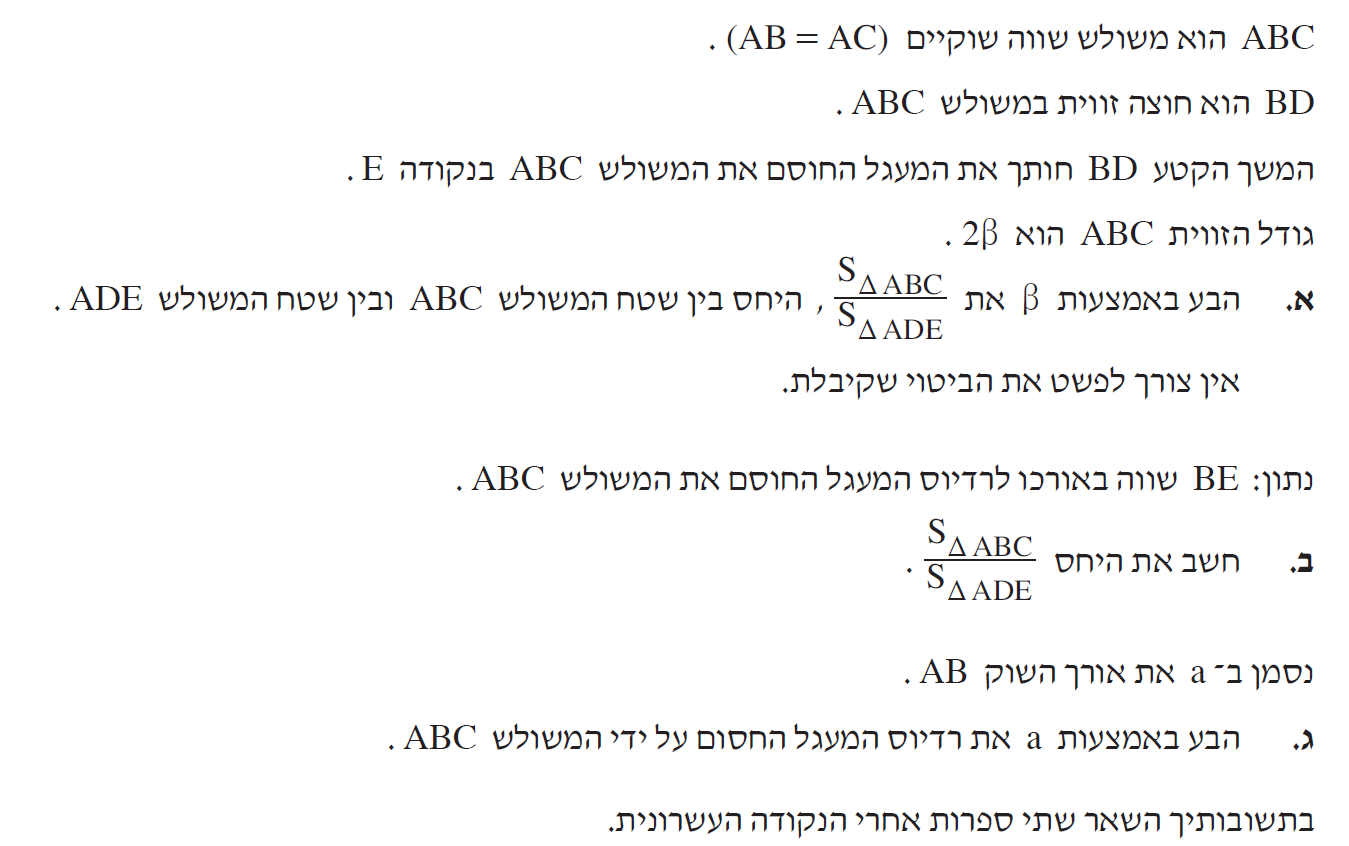
\includegraphics[width=\textwidth]{summer-2018b-5}
\end{center}

להלן התרשים עם הזוויות הנתונות ב-%
$B,C$
ולאחר חישוב הזוויות האחרות לפי סכום של זוויות של משולש. כמו כן,
$\angle EAC=\angle EBC=\beta$,
$\angle AEB=\angle ACB=2\beta$,
כי הן נשענות על אותן קשתות. התרשים נראה דחוס, אבל ציירתי אותו לפי הזוויות המתקבלות במהלך הפתרון.
\begin{center}
\selectlanguage{english}
\begin{tikzpicture}[scale=1.4]
\clip(-5mm,-5mm) rectangle +(11,2.8);
\coordinate (B) at (0,0);
\coordinate (C) at (10,0);
\path[name path=ba] (B) -- +(20:6);
\path[name path=ca] (C) -- +(160:6);
\path[name intersections={of=ca and ba,by={A}}];
\draw[thick] (A) -- node[above,xshift=24pt,yshift=10pt] {$a$} (B) -- (C) -- cycle;
\path[name path=bd] (B) -- +(10:8.5);
\tkzCircumCenter(A,B,C)\tkzGetPoint{O}
\node[draw,very thick,dotted,circle through=(A),name path=circle] (circle) at (O) {};
\path[name intersections={of=bd and ca,by={D}}];
\path[name intersections={of=bd and circle,by={E}}];
\fill (A) node[above] {$A$} circle(1.5pt);
\fill (B) node[left,xshift=-4pt] {$B$} node[above right,xshift=85pt,yshift=-1pt] {$\beta$} node[above right,xshift=85pt,yshift=16pt] {$\beta$} circle(1.5pt);
\fill (C) node[right,xshift=4pt] {$C$} node[above left,xshift=-42pt,yshift=-1pt] {$2\beta$} circle(1.5pt);
\fill (D) node[above,yshift=-2pt] {$D$} node[left,xshift=-20pt,yshift=1pt] {$3\beta$} node[below,xshift=-3,yshift=-6pt] {$180\!-\!3\beta$} circle(1.5pt);
\fill (E) node[above] {$E$} circle(1.5pt);
\draw[thick] (B) -- (D) -- (E) -- (A);
\node at ($(E)+(28pt,0pt)$) {$2\beta$};
\draw[->,thick] ($(E)+(20pt,0pt)$) -- +(-38pt,0);
\node at ($(A)+(28pt,6pt)$) {$\beta$};
\draw[->,thick] ($(A)+(27pt,1pt)$) -- +(0,-10pt);
\node at ($(A)+(-28pt,6pt)$) {$180\!-\!4\beta$};
\draw[->,thick] ($(A)+(-27pt,1pt)$) -- +(27pt,-6pt);
\end{tikzpicture}
\end{center}

\textbf{סעיף א}


$\triangle ABC$
משולש שוקיים ולכן מייד יש לנו:
\[
S_{\triangle ABC}=\frac{1}{2}\cdot a\cdot a \cdot \sin (180\!-\!4\beta)=\frac{a^2}{2}\sin 4\beta\,.
\]
כדי שהיחס יהיה ביטוי ב-%
$\beta$
בלבד, עלינו למצוא ביטוי ל-%
$S_{\triangle ADE}$
כדי ש-%
$a^2$
יצטמצם.

\np

נחפש משולשים כדי לבטא 
$AE,AD$
כביטויים ב-%
$a,\beta$
כדי ש-%
$a^2$
יצטמצם. ב-%
$\triangle ABD,\triangle ADE$
צלע אחד הוא באורך 
$a$
וצלע שני באורך
$AD,AE$.
לפי חוק הסינוסים:
\erh{14pt}
\begin{equationarray*}{rcl}
\frac{AE}{\sin \beta}&=&\frac{a}{\sin 2\beta}\\
AE&=&\frac{a\sin\beta}{\sin 2\beta}\\
\frac{AD}{\sin \beta}&=&\frac{a}{\sin 3\beta}\\
AD&=&\frac{a\sin\beta}{\sin 3\beta}\\
S_{\triangle ADE}&=&\frac{1}{2}\cdot \frac{a\sin \beta}{\sin 2\beta}\cdot\frac{a\sin\beta}{\sin 3\beta}\cdot \sin \beta\\
&=&\frac{a^2}{2}\cdot \frac{\sin^3 \beta}{\sin 2\beta\sin 3\beta}\\
\frac{S_{\triangle ABC}}{S_{\triangle ADE}}&=&\frac{\sin 4\beta\sin 2\beta\sin 3\beta}{\sin^3\beta}\,.
\end{equationarray*}

פתרון אחר משתמש בחוק הסינוסים כדי להשוות שני ביטויים עבור הרדיוס של החעגל החוסם.


\textbf{סעיף ב}

נשתמש בחוק הסינוסים על 
$\triangle ABE$
עם צלע 
$BE$,
ומ-%
$R=BE$
הרדיוס יצטמצם:
\erh{12pt}
\begin{equationarray*}{rcl}
2R&=&\frac{BE}{\sin(180\!-\!4\beta+\beta(}=\frac{BE}{\sin 3\beta}=\frac{R}{\sin 3\beta}\\
2\sin 3\beta&=&1\\
3\beta&=&30^\circ\\
\beta&=&10^\circ\,.
\end{equationarray*}
נכון שגם
$\sin 3\cdot 50 = \frac{1}{2}$,
אבל לא ייתכן שלמשולש שתי זוויות של 
$2\cdot 50=100$.

עם ערכו של 
$\beta$
נוכל לחשב את יחס השטחים:
\[
\frac{S_{\triangle ABC}}{S_{\triangle ADE}}=\frac{\sin 4\beta\sin 2\beta\sin 3\beta}{\sin^3\beta}=\frac{\sin 40\sin 20\sin 30}{\sin^3 10}=20.99^\circ\,.
\]

\np

\textbf{סעיף ג}

לפי משפט
$6$
"במשולש שווה שוקיים , חוצה זווית הראש, התיכון לבסיס והגובה לבסיס מתלכדים", כך שחוצה הזווית 
$\angle BAC$
ניצב ל-%
$BC$
בנקודה
$F$.
לפי משפט
$49$
"שלושת חוצי הזוויות של משולש נחתכים בנקודה אחת, שהיא מרכז המעגל החסום במשולש", הנקודה המסומנת 
$M$
בתרשים היא מרכז המעגל החסום.

\begin{center}
\selectlanguage{english}
\begin{tikzpicture}[scale=1.3]
\coordinate (B) at (0,0);
\coordinate (C) at (10,0);
\path[name path=ba] (B) -- +(20:6);
\path[name path=ca] (C) -- +(160:6);
\path[name intersections={of=ca and ba,by={A}}];
\draw[thick] (A) -- node[above,xshift=24pt,yshift=10pt] {$a$} (B) -- (C) -- cycle;
\path[name path=bd] (B) -- +(10:8.5);
\path[name intersections={of=bd and ca,by={D}}];
\fill (A) node[above] {$A$} circle(1.5pt);
\fill (B) node[left,xshift=-4pt] {$B$} node[above right,xshift=85pt,yshift=-1pt] {$\beta$} node[above right,xshift=85pt,yshift=16pt] {$\beta$} circle(1.5pt);
\fill (C) node[right,xshift=4pt] {$C$} circle(1.5pt);
\draw[thick] (B) -- (D);
\node at ($(A)+(-28pt,6pt)$) {$90\!-\!2\beta$};
\draw[->,thick] ($(A)+(-27pt,1pt)$) -- +(20pt,-10pt);
\coordinate (F) at ($(B)!(A)!(C)$);
\draw[rotate=90] (F) rectangle +(7pt,7pt);
\draw[thick,dashed,name path=altitude] (A) -- (F);
\path[name intersections={of=bd and altitude,by={M}}];
\fill (F) node[below] {$F$} circle(1.5pt);
\fill (M) node[above right] {$M$} circle(1.5pt);
\path (B) -- node[below] {$b$} (F);
\path (M) -- node[right] {$r$} (F);
\node[draw,very thick,dotted,circle through=(F),name path=circle] (circle) at (M) {};
\end{tikzpicture}
\end{center}
נשאר רק להשתמש בהגדרות של הפונקציות הטריגונומטריות. ב-%
$\triangle ABF$:
\erh{10pt}
\begin{equationarray*}{rcl}
\sin(90\!-\!2\beta)&=&\frac{b}{a}\\
b&=&a\cos 2\beta\,.
\end{equationarray*}

\vspace{-4ex}
ב-%
$\triangle BMF$:
\vspace{-4ex}
\erh{10pt}
\begin{equationarray*}{rcl}
\tan\beta&=&\frac{r}{b}\\
r&=&a\cos 2\beta\tan\beta\\
&=&a\cos 20\tan 10=0.1657a\,.
\end{equationarray*}

%%%%%%%%%%%%%%%%%%%%%%%%%%%%%%%%%%%%%%%%%%%%%%%%%%%%%%%%%%%%%%

\np

\section{קיץ תשע"ח מועד א}

\begin{center}
\selectlanguage{english}
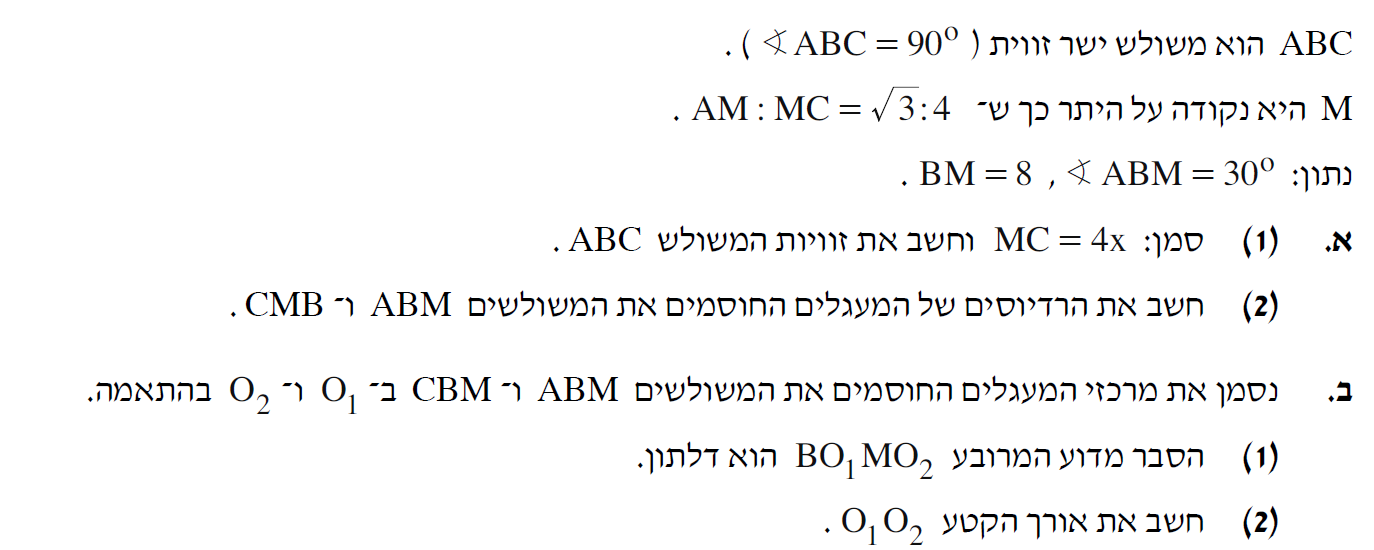
\includegraphics[width=\textwidth]{summer-2018a-5}
\end{center}

%\vspace{-1ex}

נסמן
$\angle BAM=\alpha, \angle BCM=90\!-\!\alpha$.

\vspace{-1ex}

\begin{center}
\selectlanguage{english}
\begin{tikzpicture}%[scale=1.1]
\coordinate (C) at (0,0);
\coordinate (B) at (7,0);
\path[name path=ca] (C) -- +(36:9);
\path[name path=ba] (B) -- +(90:5.5);
\path[name intersections={of=ca and ba,by={A}}];
\draw[thick] (A) -- (B) -- (C) -- cycle;
\coordinate (M) at ($(C)!{4/(sqrt(3)+4)}!(A)$);
\fill (C) node[left] {$C$} node[above right,xshift=18pt] {$90\!-\!\alpha$}circle(1.5pt);
\fill (B) node[right] {$B$} node[above left,xshift=-10pt] {$60$} node[above left,xshift=2pt,yshift=24pt] {$30$} circle(1.5pt);
\fill (A) node[right] {$A$} node[below left,xshift=2pt,yshift=-8pt] {$\alpha$} circle(1.5pt);
\fill (M) node[above left] {$M$} circle(1.5pt);
\draw[thick] (B) -- node[left,xshift=-3pt] {$8$} (M);
\path (C) -- node[above,xshift=-4pt] {$4x$} (M) -- node[above,xshift=-6pt] {$\sqrt{3}x$} (A);
\draw[rotate=90] (B) rectangle +(8pt,8pt);
\end{tikzpicture}
\end{center}

\vspace{-1ex}

\textbf{סעיף א}

$(1)$
לשני המשולשים 
$\triangle ABM,\triangle CMB$
צלע עם הנעלם
$x$,
זווית ידועה אחת, וזווית שנייה עם הנעלם 
$\alpha$.
מחוק הסינוסים נקבל שתי משוואות עם שני הנעלמים שאפשר לפתור אתכדי לקבל משוואה אחת עם הנעלם
$\alpha$
בלבד:
\erh{14pt}
\begin{equationarray*}{rcl}
\frac{\sqrt{3}x}{\sin 30}&=&\frac{8}{\sin\alpha}\\
x&=&\frac{8\sin 30}{\sqrt{3}x\sin\alpha}\\
\frac{4x}{\sin 60}&=&\frac{8}{\sin (90\!-\!\alpha)}\\
x&=&\frac{8\sin 60}{4x\cos\alpha}
\end{equationarray*}

\np

\erh{10pt}
\begin{equationarray*}{rcl}
%\frac{8\sin 30}{\sqrt{3}\sin\alpha}&=&\frac{8\sin 60}{4\sin (90\!-\!\alpha)}\\
\frac{1}{2\sqrt{3}\sin\alpha}&=&\frac{\sqrt{3}}{4\cdot 2\cos \alpha}\\
\tan \alpha&=&\frac{4}{3}\,.
\end{equationarray*}
לכן,
$\angle BAC=\alpha = 53.13$,
ולא נשכח לרשום גם 
$\angle BCA=90\!-\!\alpha=36.87$.


$(2)$
לפי חוק הסינוסים עבור 
$\triangle ABM$, $\triangle CMB$:
\erh{8pt}
\begin{equationarray*}{rcl}
2R_1&=&\frac{8}{\sin\alpha}\\
R_1&=&5\\
2R_2&=&\frac{8}{\sin(90\!-\!\alpha)}\\
R_2&=&20/3\,.
\end{equationarray*}

\vspace{-3ex}

\textbf{סעיף ב}

$(1)$
נצייר התרשים חדש עם המעגלים החוסמים. ניתן לראות ש-%
$O_1M=O_1B$
כי הם רדיוסים של המעגל החוסם את
$\triangle ABM$,
ו-%
$O_2M=O_2B$
כי הם רדיוסים של המעגל החוסם את
$\triangle CBM$.
לפי ההגדרה מרובע עם שני זוגות של צלעות שכנים שהם שווים הוא דלתון.
\begin{center}
\selectlanguage{english}
\begin{tikzpicture}%[scale=1.1]
\clip (-6mm,-5mm) rectangle +(11,6);
\coordinate (C) at (0,0);
\coordinate (B) at (7,0);
\path[name path=ca] (C) -- +(36:9);
\path[name path=ba] (B) -- +(90:5.5);
\path[name intersections={of=ca and ba,by={A}}];
\draw[thick] (A) -- (B) -- (C) -- cycle;
\coordinate (M) at ($(C)!{4/(sqrt(3)+4)}!(A)$);
\fill (C) node[left] {$C$} circle(1.5pt);
\fill (B) node[right] {$B$} circle(1.5pt);
\fill (A) node[right] {$A$} circle(1.5pt);
\fill (M) node[above left] {$M$} circle(1.5pt);
\draw[thick] (B) -- (M);
\tkzCircumCenter(A,B,M)\tkzGetPoint{O1}
\tkzCircumCenter(C,B,M)\tkzGetPoint{O2}
\fill (O1) node[above right] {$O_1$} circle(1.5pt);
\fill (O2) node[above left] {$O_2$} circle(1.5pt);
\node [draw,thick,dotted,circle through=(M)] (circle) at (O1) {};
\node [draw,thick,dotted,circle through=(M)] (circle) at (O2) {};
\draw[thick] (O1) -- node[right] {$R_1$} (B) -- node[below,yshift=-3pt] {$R_2$} (O2) -- node[left] {$R_2$} (M) -- node[above] {$R_1$} cycle;
\draw[thick,name path=diagonal1] (O1) -- (O2);
\path[name path=diagonal2] (M) -- (B);
\path[name intersections={of=diagonal1 and diagonal2,by={E}}];
\fill (E) node[left,xshift=-3pt,yshift=2pt] {$E$} circle(1.5pt);
\draw[rotate=32] (E) rectangle +(7pt,7pt);
\path (M) -- node[left] {$4$} (E) -- node[left,xshift=-3pt,yshift=4pt] {$4$} (B);
\end{tikzpicture}
\end{center}

$(2)$
לפי משפט
$21$
"האלכסון הראשי בדלתון חוצה את זוויות הראש, חוצה את האלכסון השני ומאונך לו", 
$MB\perp O_1O_2$
וחוצה אותו. את האורך של
$O_1O_2$
ניתן לחשב כסכום האורכים ממרכזי המעגלים ועד לנקודת החיתוך של האלכסונים. נשמתמש במשפט פיתגורס:
\erh{16pt}
\begin{equationarray*}{rcl}
O_1O_2=O_1E+O_2E&=&\sqrt{R_1^2-16} + \sqrt{R_2^2-16}\\
&=&\sqrt{5^2-16} + \sqrt{\left(\frac{20}{3}\right)^2-16}\\
&=&3+\frac{16}{3}=\frac{25}{3}\,.
\end{equationarray*}

%%%%%%%%%%%%%%%%%%%%%%%%%%%%%%%%%%%%%%%%%%%%%%%%%%%%%%%%%%%%%%

\np


\section{חורף תשע"ח}

\begin{center}
\selectlanguage{english}
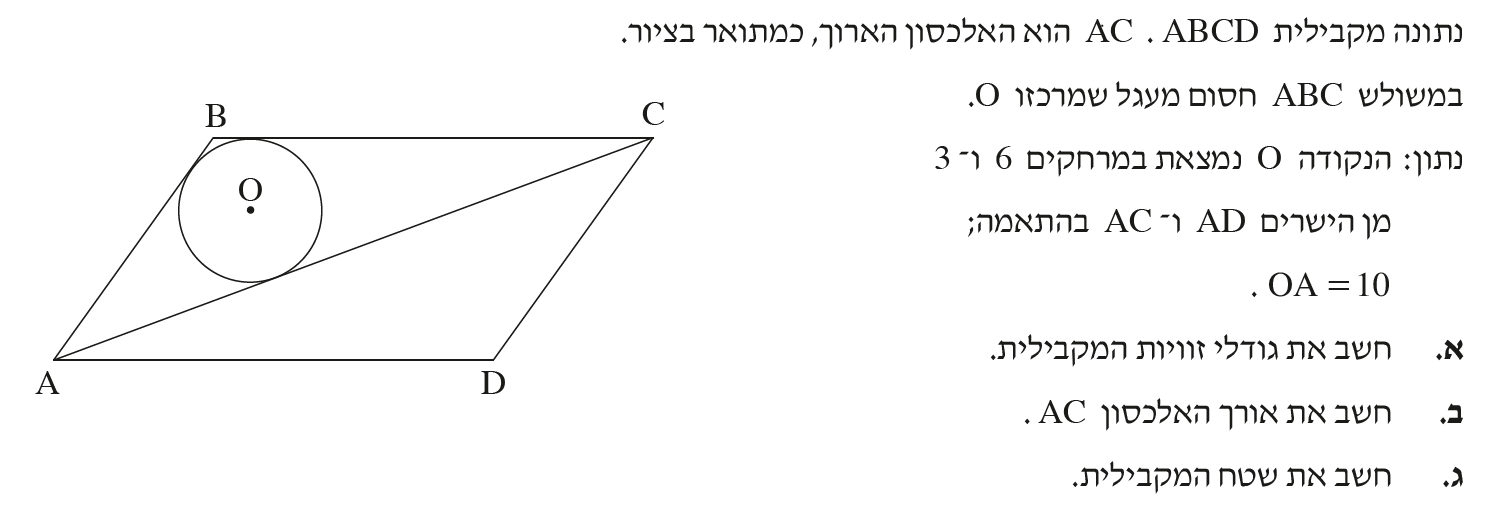
\includegraphics[width=\textwidth]{winter-2018-5}
\end{center}

\vspace{-1ex}

$E,F$
הן נקודות המפגש של האנכים מ-%
$O$
עם 
$AC,AD$.
לפי משפט
$49$
"שלושת חוצי הזוויות של משולש נחתכים בנקודה אחת, שהיא מרכז המעגל החסום במשולש", 
$AO,CO$
הם חוצי הזוויות
$BAC,BCA$,
בהתאמה. המונח "חוצה זוויות" נתפס לי בראש ו"פתרתי" את הבעיה תוך הנחה שאלכסון של מקבילית חוצה את הזווית:
$\angle BAC=\angle CAD$.
כמובן שזה נכון רק עבור מעוין.

נסמן את הזוויות בנקודה
$A$
עבור המשולשים ישר-זווית
$\triangle AOE, \triangle AOF$
שנוצרו על ידי האנכים:
$\alpha=\angle OAE,\beta=\angle OAF$.

\vspace{-2ex}

\begin{center}
\selectlanguage{english}
\begin{tikzpicture}%[scale=1.1]
\clip (-12mm,-5.5mm) rectangle +(12.5,5);
\coordinate (A) at (0,0);
\coordinate (D) at (8,0);
\coordinate (B) at (54:4.5);
\coordinate (C) at ($(D)+(54:4.5)$);
\fill (A) node[below] {$A$} circle(1.5pt);
\fill (B) node[above] {$B$} circle(1.5pt);
\fill (C) node[above] {$C$} circle(1.5pt);
\fill (D) node[below] {$D$} circle(1.5pt);
\draw[thick] (D) -- (A) -- (B) -- (C) -- cycle;
\draw[thick] (A) -- (C);
\tkzInCenter(A,B,C)\tkzGetPoint{O}
\fill (O) node[above] {$O$} circle(1.5pt);
\node[draw,thick,circle through=($(B)!(O)!(C)$),name path=circle] at (O) {};
\draw[thick,dashed] (A) -- node[left,near end,xshift=10pt,yshift=12pt] {$10$} (O) -- (C);
\coordinate (E) at ($(A)!(O)!(C)$);
\coordinate (F) at ($(A)!(O)!(D)$);
\fill (E) node[below right] {$E$} circle(1.5pt);
\fill (F) node[below] {$F$} circle(1.5pt);
\draw[thick,dashed] (E) -- node[right,near end] {$3$} (O) -- node[right,near end] {$6$} (F);
\draw[rotate=19] (E) rectangle +(7pt,7pt);
\draw (F) rectangle +(7pt,7pt);
\draw[thick] ($(A)+(20mm,0)$) arc[start angle=0,end angle=37,radius=20mm];
\node[right,xshift=54pt,yshift=12pt] at (A) {$\beta$};
\node[above right,xshift=34pt,yshift=14pt] at (A) {$\alpha$};
\node[above right,xshift=28pt,yshift=28pt] at (A) {$\alpha$};
\node at (-2mm,2.5) {$\angle OAF=\beta$};
\end{tikzpicture}
\end{center}

\vspace{-2ex}

\textbf{סעיף א}

לפי התרשים
$\angle BAD=\alpha+\beta$.
נחשב
$\alpha,\beta$
מהפונקציות הטריגונומטריות במשולשים ישר-זווית:
\erh{12pt}
\begin{equationarray*}{rcl}
\sin \alpha &=& 3/10\\
\alpha &=& 17.46\\
\sin \beta &=& 6/10\\
\beta &=& 36.87\\
\angle BCD =\angle BAD&=& \alpha+\beta=54.33\\
\angle ABC =\angle ADC&=& \frac{360-2(\alpha+\beta)}{2}=125.67\,.
\end{equationarray*}

\np


\textbf{סעיף ב}

האלכסון
$AC$
הוא צלע של
$\triangle ABC$
והזוויות שלו ידועים, אבל אי-אפשר להשתמש בחוק הסינוסים כי אורכי הצלעות לא ידועים. מהתרשים רואים שהאלכסון מורכב משני קטעי קו
$AE,EC$
שהם צלעות של משולשים ישר-זווית
$\triangle AOE, \triangle COE$.
$AE$
מתקבל ממשפט פיתגורס:
\[
AE = \sqrt{10^2-3^2}=9.54\,.
\]
נשתמש בחוק הסינוסים ב-%
$\triangle COE$
)ונימנע מהפיתוי לקבוע ש-%
$\angle OCE=\alpha$(.
לפי זוויות מתחלפות במקבילית
$\angle BCA=\angle CAD=\beta-\alpha$
ו:

\vspace{-2ex}

\erh{12pt}
\begin{equationarray*}{rcl}
\angle OCE=\frac{\angle BCA}{2}&=&\frac{\beta-\alpha}{2}\\
&=&\frac{36.87-17.46}{2}=9.71\\
\angle COE &=& 180-90-\angle OCE=80.29\\
\frac{EC}{\sin 80.29}&=& \frac{3}{\sin 9.71}\\
EC&=&17.54\\
AC=AE+EC&=&9.54+17.54=27.08\,.
\end{equationarray*}

\vspace{-2ex}

\textbf{סעיף ג}

שטח של מקבילית הוא הבסיס כפול הגובה:

\begin{center}
\selectlanguage{english}
\begin{tikzpicture}[scale=.7]
\coordinate (A) at (0,0);
\coordinate (B) at (54:4.5);
\coordinate (D) at (8,0);
\coordinate (C) at ($(D)+(54:4.5)$);
\fill (A) node[below] {$A$} node[above right,xshift=46pt,yshift=0pt] {$\beta-\alpha$} node[above right,xshift=16pt,yshift=10pt] {$2\alpha$} circle(1.5pt);
\fill (B) node[above] {$B$} circle(1.5pt);
\fill (C) node[above] {$C$} circle(1.5pt);
\fill (D) node[below] {$D$} circle(1.5pt);
\draw[thick] (D) -- node[below] {$b$} (A) -- node[above,yshift=2pt] {$27.08$} (C) -- cycle;
\draw[thick] (A) -- (B) -- (C);
\coordinate (H) at ($(A)!(C)!(D)$);
\fill (H) node[below] {$H$} circle(1.5pt);
\draw[rotate=90] (H) rectangle +(10pt,10pt);
\draw[thick,dashed] (D) -- (H) -- node[right] {$h$} (C);
%\node[above right,xshift=46pt,yshift=0pt] at (A) {$\beta-\alpha$};
\node[above left,xshift=-2pt,yshift=2pt] at (D) {$125.67$};
\node[below left,xshift=-16pt,yshift=-12pt] at (C) {$2\alpha$};
\end{tikzpicture}
\end{center}

\vspace{-4ex}

\erh{12pt}
\begin{equationarray*}{rcl}
\frac{b}{\sin 2\alpha}&=&\frac{27.08}{\sin 125.67}\\
b&=&19.08\\
\sin (\beta-\alpha) &=& \frac{h}{27.08}\\
h&=&9\\
S_{ABCD}=bh&=&171.71\,.
\end{equationarray*}

\vspace{-2ex}


אפשרות אחרת היא להשתמש בנוסחה הטריגונומטרית כדי לחשב 
$S_{\triangle ABC}$
ולהכפיל בשניים.

%%%%%%%%%%%%%%%%%%%%%%%%%%%%%%%%%%%%%%%%%%%%%%%%%%%%%%%%%%%%%%

\np

\section{קיץ תשע"ז מועד ב}

\begin{center}
\selectlanguage{english}
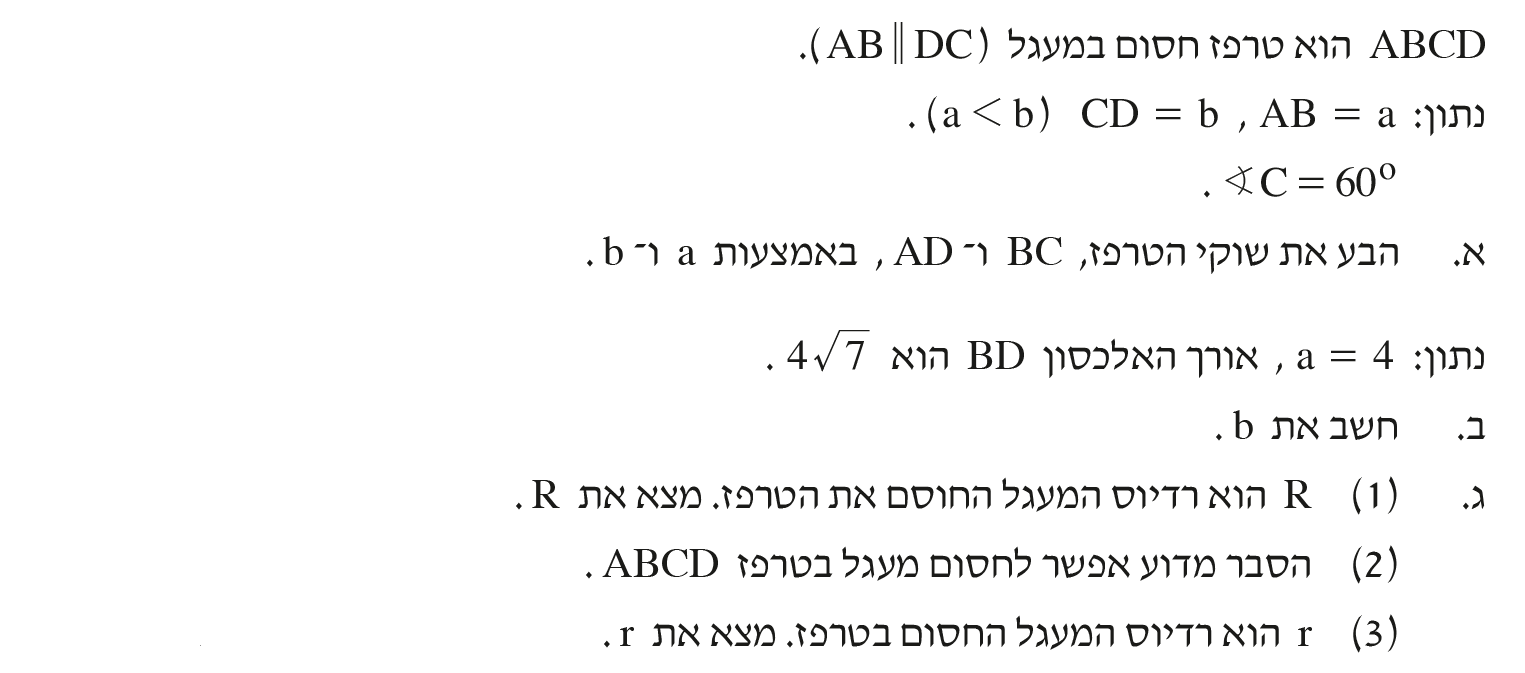
\includegraphics[width=\textwidth]{summer-2017b-5}
\end{center}

\vspace{-1ex}

\textbf{סעיף א}


לפי משפט
$56$
"ניתן לחסום מרובע במעגל אם ורק אם סכום זוג זוויות נגדיות שווה ל-%
$180$",
ולכן
$\angle DAB=120$.
נוריד גבהים מ-%
$A,B$
ל-%
$CD$
החותחכים אותו ב-%
$E,F$.
$\triangle AED,\triangle BFC$
הם משולשים ישר-זווית. בתרשים השלמנו את הזוויות במשולשים ל-%
$180$.
לפי משפט
$40$
"טרפז בו הזוויות שליד אותו בסיס שוות זו לזו הוא טרפז שווה שוקיים", 
$ABCD$
שווה שוקיים.

%\vspace{-1ex}

\begin{center}
\selectlanguage{english}
\begin{tikzpicture}[scale=1.1]
\clip (-.5,-.5) rectangle +(9,4.25);
\draw[thick] (0,0) coordinate (D) node[below left] {$D$} -- node[below] {$b$} (8,0) coordinate (C) node[below right] {$C$};
\fill (C) node[above left,xshift=-4pt] {$60$} circle(1.5pt);
\fill (D) node[above right,xshift=4pt] {$60$} circle(1.5pt);
\path[name path=s1] (D) -- +(60:4);
\path[name path=s2] (C) -- +(120:4);
\path[name path=top] (1,3) -- (7,3);
\path[name intersections={of=s1 and top,by={A}}];
\path[name intersections={of=s2 and top,by={B}}];
%\fill (A) node[above left] {$A$} node[below right] {$120$} circle(1.5pt);
\fill (A) node[above left] {$A$} node[below right] {$90$} node[below,xshift=-8pt,yshift=-22pt] {$30$}  circle(1.5pt);
%\fill (B) node[above right] {$B$} node[below left] {$120$} circle(1.5pt);
\fill (B) node[above right] {$B$} node[below left] {$90$}  node[below,xshift=8pt,yshift=-22pt] {$30$} circle(1.5pt);
\draw[thick] (D) -- node[left] {$s$} (A) -- node[above] {$a$} (B) -- node[right] {$s$} (C);
\tkzCircumCenter(A,B,C)\tkzGetPoint{O}
\tkzDrawCircle[thick,dotted,name path=circle](O,A)
%\fill (O) circle(1.5pt);
\coordinate (E) at (D-|A);
\fill (E) node[below] {$E$} circle(1.5pt);
\draw[thick,dashed] (A) -- (E);
\draw (E) rectangle +(8pt,8pt);
\coordinate (F) at (D-|B);
\fill (F) node[below] {$F$} circle(1.5pt);
\draw[thick,dashed] (B) -- (F);
\draw[rotate=90] (F) rectangle +(8pt,8pt);
\draw[dashed] (A) -- node[below,xshift=-4pt] {$c$} (C);
\end{tikzpicture}
\end{center}

%\vspace{-1ex}

$AE=BF$
כך ש-%
$\triangle AED\cong\triangle BFC$.
מכאן:

\vspace{-2ex}

\erh{6pt}
\begin{equationarray*}{rcl}
\cos 60 &=& \frac{(b-a)/2}{s}=\frac{1}{2}\\
s&=&b-a\,.
\end{equationarray*}

\vspace{-4ex}

פתרון אחר משתמש בחוק הקוסינוסים על 
$\triangle ACD,\triangle ACB$.
נסמן ב-%
$c$
את אורך האלכסון
$AC$.

\vspace{-2ex}

\erh{2pt}
\begin{equationarray*}{rcl}
c^2 &=& s^2+b^2-2sb\cos 60\\
&=& s^2-sb+b^2\\
c^2 &=& s^2+a^2-2sa\cos 120\\
&=& s^2+sa+a^2
\end{equationarray*}
\vspace{-3ex}

נשווה את שתי הנוסחאות ל-%
$c^2$
ונפתור עבור 
$s$:

\np

\erh{2pt}
\begin{equationarray*}{rcl}
s(b+a)&=&b^2-a^2=(b+a)(b-a)\\
s&=&b-a\,.
\end{equationarray*}

\vspace{-4ex}

\textbf{סעיף ב}

שקלתי להשתמש בחוק הסינוסים במשלוש
$\triangle ADB$:
פעם אחת לחשב 
$\angle ADB$
ופעם שנייה לחשב את
$s$.
עדיף להשתמש בחוק הקוסינוסים ב-%
$\triangle ADB$
כי אנו יודעים ש-%
$s=b-a=b-4$:
\erh{3pt}
\begin{equationarray*}{rcl}
(4\sqrt{7})^2&=&4^2+(b-4)^2-2\cdot 4\cdot (b-4)\cdot \cos 120\\
b^2-4b-96&=&0\\
(b-12)(b+8)&=&0\\
b&=&12\,.
\end{equationarray*}

\vspace{-2ex}

\begin{center}
\selectlanguage{english}
\begin{tikzpicture}[scale=1.1]
\clip (-.5,-.5) rectangle +(9,4.25);
\draw[thick] (0,0) coordinate (D) node[below left] {$D$} -- node[above] {$b$} (8,0) coordinate (C) node[below right] {$C$};
\fill (C) node[above left,xshift=-4pt] {$60$} circle(1.5pt);
\fill (D) circle(1.5pt);
\path[name path=s1] (D) -- +(60:4);
\path[name path=s2] (C) -- +(120:4);
\path[name path=top] (1,3) -- (7,3);
\path[name intersections={of=s1 and top,by={A}}];
\path[name intersections={of=s2 and top,by={B}}];
\fill (A) node[above left] {$A$} node[below right] {$120$} circle(1.5pt);
\fill (B) node[above right] {$B$} circle(1.5pt);
\draw[thick] (D) -- node[left,xshift=-14pt] {$b-4$} (A) -- node[above] {$4$} (B) -- node[right,xshift=14pt] {$b-4$} (C);
\tkzCircumCenter(A,B,C)\tkzGetPoint{O}
\tkzDrawCircle[thick,dotted,name path=circle](O,A)
\fill (O) circle(3pt);
\coordinate (E) at (D-|A);
\coordinate (F) at (D-|B);
\fill (F) node[below] {$F$} circle(1.5pt);
\draw[thick,dashed] (B) -- node[left] {$2r$} (F);
\draw[rotate=90] (F) rectangle +(8pt,8pt);
\draw[thick,dashed] (B) -- node[below] {$4\sqrt{7}$} (D);
\end{tikzpicture}
\end{center}


\textbf{סעיף ג}

$(1)$
שימו לב שהאלכסון
$BD$
הוא 
\textbf{לא}
הקוטר של המעגל החוסם שמסומן בנקודה השחורה הגדולה. לפי חוק הסינוסים ב-%
$\triangle ADB$:
\[
R = \frac{4\sqrt{7}}{2\sin 120} = \frac{4\sqrt{7}}{\sqrt{3}}=6.11\,.
\]

\vspace{-1ex}

$(2)$
לפי משפט
$57$,
"מרובע קמור חוסם מעגל אם ורק אם סכום שתי צלעות נגדיות שווה לסכום שתי הצלעות הנגדיות האחרות":

\vspace{-4ex}

\erh{3pt}
\begin{equationarray*}{rcl}
a+b&\stackrel{?}{=}&s+s\\
a+b&\stackrel{?}{=}&(b-a)+(b-a)\\
3a&\stackrel{?}{=}&b\\
3\cdot 4&=&12\,.
\end{equationarray*}

\vspace{-4ex}

$(3)$
$AB,CD$
הם משיקים מקבילים למעגל החסום, ולכן
$BF=2r$:
\erh{14pt}
\begin{equationarray*}{rcl}
\sin 60 &=& \frac{2r}{s}=\frac{2r}{b-a}=\frac{2r}{8}\\
r&=&\frac{1}{2}\cdot\frac{\sqrt{3}}{2}\cdot 8 = 2\sqrt{3}=3.464\,.
\end{equationarray*}

%%%%%%%%%%%%%%%%%%%%%%%%%%%%%%%%%%%%%%%%%%%%%%%%%%%%%%%%%%%%%%


\np


\section{קיץ תשע"ז מועד א}

\begin{center}
\selectlanguage{english}
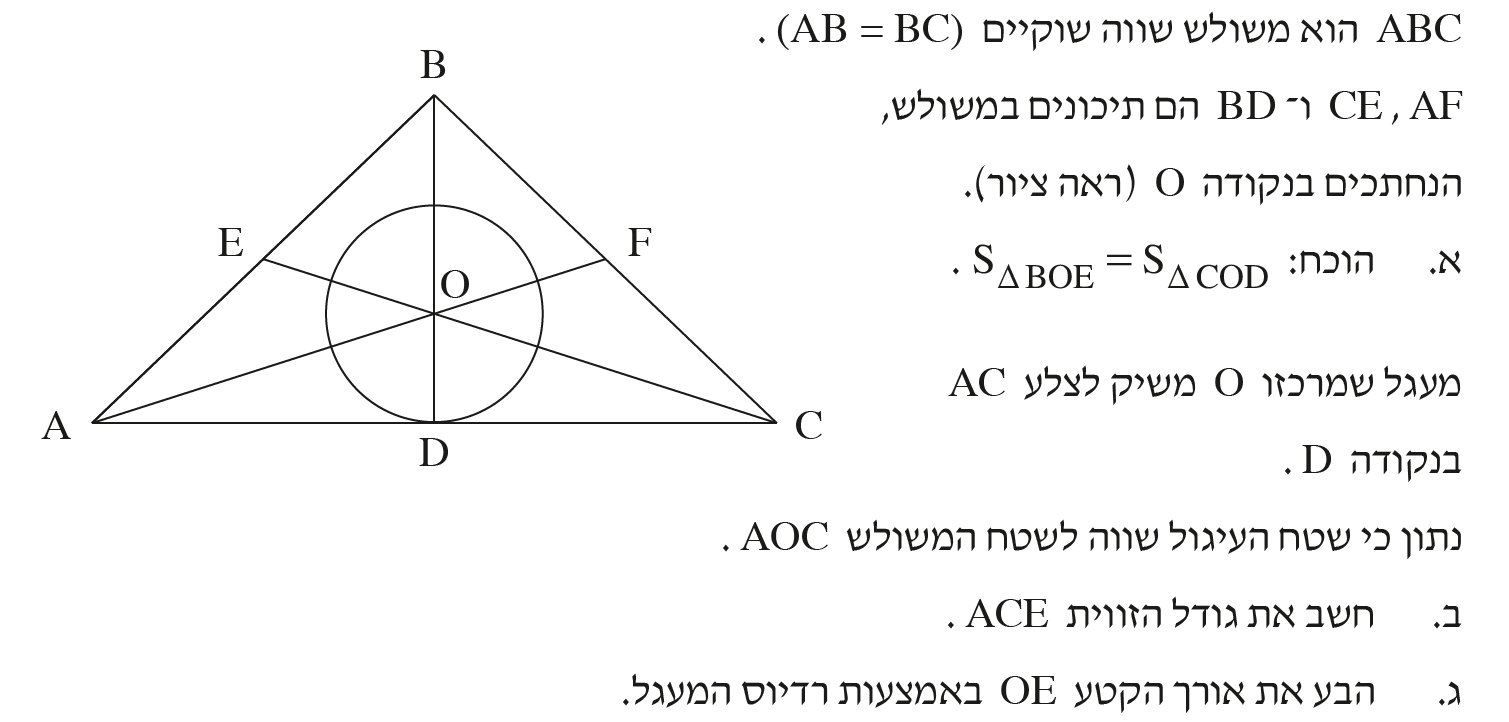
\includegraphics[width=\textwidth]{summer-2017a-5}
\end{center}

\vspace{-2ex}

\textbf{סעיף א}

נסמן בתרשים לפי: 
$\triangle ABC$
שווה שוקיים,
$AF,BD,CF$
תיכונים. משפט
$46$
"נקודת חיתוך התיכונים מחלקת כל תיכון ביחס 
$2\!:\!1$".
$AF=CE$
כי
$\triangle CAF\cong \triangle ACE$
לפי צ.ז.צ. כי 
$\triangle ABC$
שווה-שוקיים.

\vspace{-1ex}

\begin{center}
\selectlanguage{english}
\begin{tikzpicture}[scale=1.1]
\draw[thick] (0,0) coordinate (A) node[left] {$A$} -- (8,0) coordinate (C) node[right] {$C$} -- (4,4.5) coordinate (B) node[above] {$B$} -- cycle;
\fill (A) circle(1.5pt);
\fill (B) circle(1.5pt);
\fill (C) circle(1.5pt);
\coordinate (D) at ($(A)!.5!(C)$);
\coordinate (E) at ($(A)!.5!(B)$);
\coordinate (F) at ($(C)!.5!(B)$);
\fill (D) node[below] {$D$} circle(1.5pt);
\fill (E) node[left,xshift=-2pt,yshift=2pt]  {$E$} circle(1.5pt);
\fill (F) node[right,xshift=2pt,yshift=2pt] {$F$} circle(1.5pt);
\draw (D) rectangle +(8pt,8pt);
\draw[thick,name path=af] (A) -- (F);
\draw[thick,name path=ce] (C) -- (E);
\draw[thick,name path=bd] (B) -- (D);
\path[name intersections={of=af and ce,by={O}}];
\fill (O) node[above right,yshift=2pt] {$O$} node[above left,xshift=2pt,yshift=2pt] {$\alpha$} node[below right,xshift=-2pt,yshift=-2pt] {$\alpha$} circle(1.5pt);
\path (A) -- node[below] {$a/2$} (D) -- node[below] {$a/2$} (C);
\path (A) -- node[left] {$b/2$} (E) -- node[left] {$b/2$} (B);
\path (C) -- node[right] {$b/2$} (F) -- node[right] {$b/2$} (B);
\path (B) -- node[right] {$2r$} (O) -- node[right] {$r$} (D);
\path (A) -- node[above] {$2c$} (O) -- node[below] {$c$} (F);
\path (C) -- node[above] {$2c$} (O) -- node[below] {$c$} (E);
\draw[thick,dashed,name path=ef] (E) -- (F);
\path[name intersections={of=ef and bd,by={G}}];
\fill (G) node[above left] {$G$} circle(1.5pt);
\draw (G) rectangle +(8pt,8pt);
\end{tikzpicture}
\end{center}

\vspace{-1ex}


נשתמש במשפט
$91$
"משפט תאלס המורחב: ישר המקביל לאחת מצלעות המשולש חותך את שתי הצלעות האחרות או את המשכיהן בקטעים פרופורציוניים", כך ש-%
$EF=\displaystyle\frac{AC}{2}=\frac{a}{2}$.
$\triangle EBF$
גם הוא שווה-שוקיים, ולכן,
$EG=\displaystyle\frac{EF}{2}=\frac{a}{4}$.

\vspace{-1ex}

\erh{16pt}
\begin{equationarray*}{rcl}
S_{BOE}&=&\frac{1}{2}\cdot \frac{a}{4}\cdot BG+\frac{1}{2}\cdot \frac{a}{4}\cdot GO =\frac{a}{8}(BG+GO)=\frac{a}{8}\cdot 2r= \frac{ar}{4}\\
S_{COD} &=& \frac{1}{2}\cdot r\cdot \frac{a}{2} =\frac{ar}{4}\,.
\end{equationarray*}

\np

פתרון אחר מתקבל מהנוסחה הטריגונומטרית לשטח עם הזוויות הקודקודיות 
$\alpha$:

\vspace{-4ex}

\erh{14pt}
\begin{equationarray*}{rcl}
S_{BOE}&=&\frac{1}{2}\cdot 2r\cdot c\cdot \sin \alpha\\
S_{COD}&=&\frac{1}{2}\cdot r\cdot 2c\cdot \sin \alpha\,.
\end{equationarray*}

\vspace{-3ex}

פתרון זה הרבה יותר קל רק קשה לי להיגמל מגישה גיאומטרית לחשב שטח מבסיס וגובה!

\medskip

\textbf{סעיף ב}

\begin{center}
\selectlanguage{english}
\begin{tikzpicture}[scale=1.1]
\draw[thick] (0,0) coordinate (A) node[left] {$A$} -- (8,0) coordinate (C) node[right] {$C$} -- (4,4.5) coordinate (B) node[above] {$B$} -- cycle;
\fill (A) circle(1.5pt);
\fill (B) circle(1.5pt);
\fill (C) node[left,xshift=-35pt,yshift=6pt] {$\beta$} circle(1.5pt);
\coordinate (D) at ($(A)!.5!(C)$);
\coordinate (E) at ($(A)!.5!(B)$);
\coordinate (F) at ($(C)!.5!(B)$);
\fill (D) node[below] {$D$} circle(1.5pt);
\fill (E) node[left,xshift=-2pt,yshift=2pt]  {$E$} circle(1.5pt);
\fill (F) node[right,xshift=2pt,yshift=2pt] {$F$} circle(1.5pt);
\draw (D) rectangle +(8pt,8pt);
\draw[thick,name path=af] (A) -- (F);
\draw[thick,name path=ce] (C) -- (E);
\draw[thick,name path=bd] (B) -- (D);
\path[name intersections={of=af and ce,by={O}}];
\fill (O) node[above right,yshift=2pt] {$O$} circle(1.5pt);
\path (A) -- node[below] {$a/2$} (D) -- node[below] {$a/2$} (C);
%\path (A) -- node[left] {$b/2$} (E) -- node[left] {$b/2$} (B);
%\path (C) -- node[right] {$b/2$} (F) -- node[right] {$b/2$} (B);
\path (B) -- node[right,near start] {$2r$} (O) -- node[right] {$r$} (D);
\path (A) -- node[above] {$2c$} (O) -- node[below] {$c$} (F);
\path (C) -- node[above] {$2c$} (O) -- node[below] {$c$} (E);
\node [draw,thick,circle through=(D),name path=circ] (circle) at (O) {};
\end{tikzpicture}
\end{center}

\vspace{-2ex}
נתון:
\vspace{-4ex}

\erh{14pt}
\begin{equationarray*}{rcl}
S_O&=&\pi r^2 = \frac{1}{2} ar = S_{AOC}\\
a &=& 2\pi r\,.
\end{equationarray*}

\vspace{-4ex}

נציב עבור 
$a$
בחישוב פונקציה טריגונומטרית עבור הזווית
$\beta = \angle ACE$:
\erh{14pt}
\begin{equationarray*}{rcl}
\tan \beta &=& \frac{r}{a/2} = \frac{2r}{2\pi r}=\frac{1}{\pi}\\
\beta &=& \arctan \frac{1}{\pi}= 17.66^\circ\,.
\end{equationarray*}

\vspace{-2ex}

\textbf{סעיף ג}

בתרשים סימנו
$OE=c$.
נחשב פונקציה טריגונומטרית עבור הזווית
$\beta$
ב-%
$\triangle COD$:

\vspace{-2ex}

\erh{14pt}
\begin{equationarray*}{rcl}
\sin \beta &=& \frac{r}{2c}\\
c &=& \frac{r}{2\sin \beta}\\
&=& 1.648r\,.
\end{equationarray*}

%%%%%%%%%%%%%%%%%%%%%%%%%%%%%%%%%%%%%%%%%%%%%%%%%%%%%%%%%%%%%%

\np



\section{חורף תשע"ז}

\begin{center}
\selectlanguage{english}
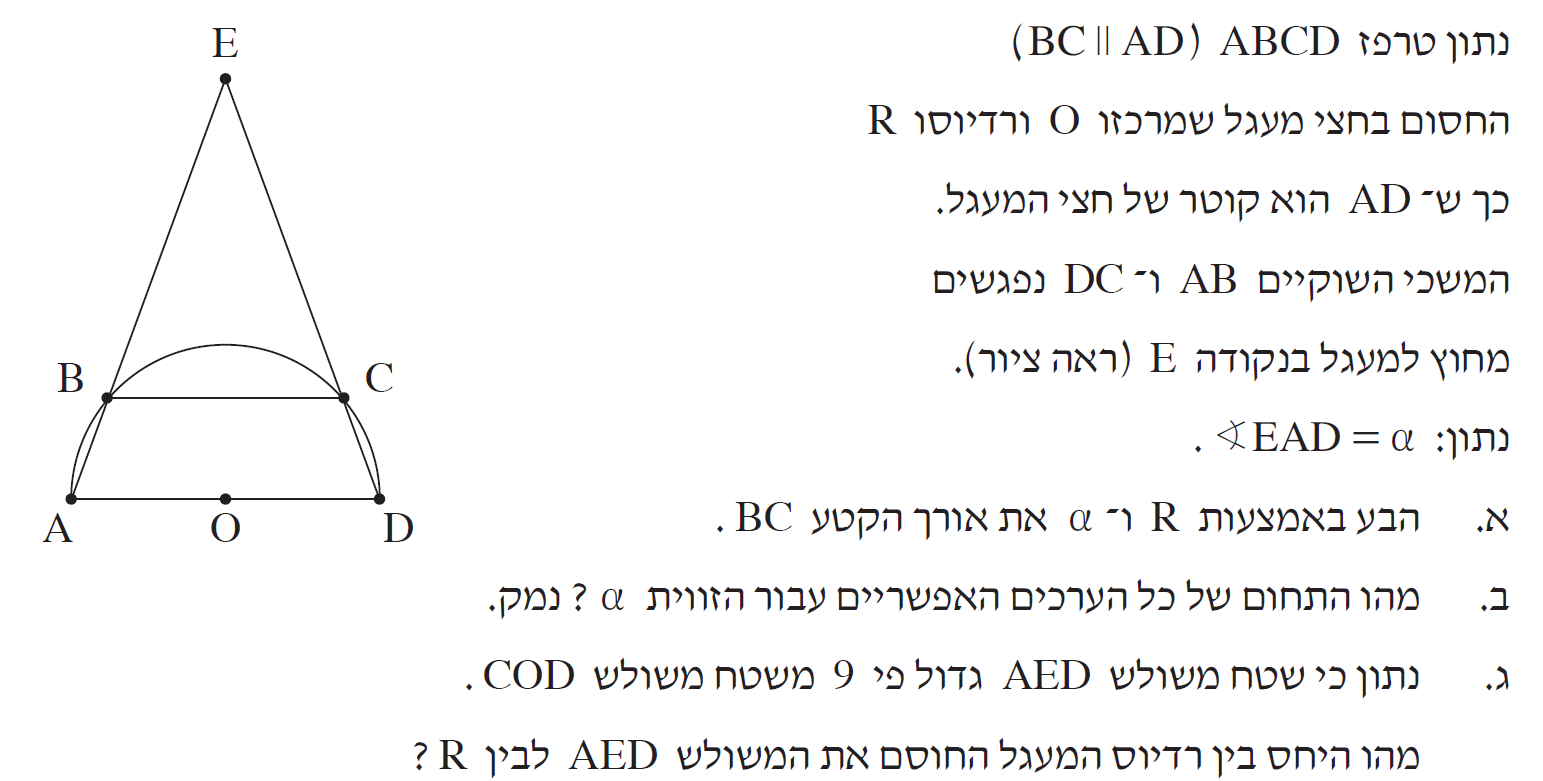
\includegraphics[width=\textwidth]{winter-2017-5}
\end{center}

\textbf{סעיף א}

להלן ההצדקה לסימונים של הזוויות בתרשים להלן. הרדיוסים של המעגל שווים
$OA=OB=OC=OD=R$,
לכן
$\triangle ABO$
שווה-שוקיים, ו-%
$\angle BAO=\angle ABO=\alpha$.
כדי להשלים זוויות של
$\triangle ABO$
ל-%
$180$,
$\angle AOB=180-2\alpha$
שנסמן
$\beta$.
$\angle BCO=\angle AOB=\beta$
לפי זוויות מתחלפות, ו-%
$\angle BCO=\angle CBO=\beta$
כי
$\triangle BOC$
שווה שוקיים. נשלים את הזוויות של
$\triangle BOC$
ונקבל
$\angle BOC=180-2\beta$
שנסמן 
$\gamma$.
לפי זוויות מתחלפות
$\angle COD=\angle BCO=\beta$.
$\triangle COD$
שווה שוקיים, ולכן
$\angle CDO=\angle OCD=(180-\beta)/2=\alpha$.

אפשר גם להשתמש במשפט
$56$
"ניתן לחסום מרובע במעגל אם ורק אם סכום זוג זוויות נגדיות שווה ל-%
$180^\circ$.
לאחר שהסקנו ש-%
$\angle OAB=\angle ABO=\alpha$
ו-%
$\angle AOB=\angle CBO=180-2\alpha=\beta$,
אפשר לחשב ש-%
$\angle CDO=\alpha$
ומשם את שאר הזוויות.
\vspace{-1ex}

\begin{center}
\selectlanguage{english}
\begin{tikzpicture}%[scale=1.1]
\coordinate (A) at (0,0);
\draw[thick] (A) -- ++(6,0) coordinate (D) -- ++(120:3) coordinate (C);
\draw[thick] (A) -- ++(60:3) coordinate (B) -- node[above] {$a$} (C);
\coordinate (O) at (3,0);
\draw[thick] (D) arc(0:180:3);
\path[name path=ae] (A) -- ($(A) ! 2.1 ! (B)$);
\path[name path=de] (D) -- ($(D) ! 2.1 ! (C)$);
\path[name intersections={of=ae and de,by={E}}];
\draw[thick] (B) -- (E) -- (C);
\fill (A) node[below left] {$A$} node[above right,xshift=4pt] {$\alpha$} circle(1.5pt);
\fill (B) node[above left] {$B$} node[below,yshift=-6pt] {$\alpha$} node[below right,xshift=8pt] {$\beta$} circle(1.5pt);
\fill (C) node[above right] {$C$} node[below,yshift=-6pt] {$\alpha$} node[below left,xshift=-8pt] {$\beta$} circle(1.5pt);
\fill (D) node[below right] {$D$}  node[above left,xshift=-4pt] {$\alpha$} circle(1.5pt);
\fill (E) node[above] {$E$} circle(1.5pt);
\fill (O) node[below] {$O$} node[above left,xshift=-8pt] {$\beta$} node[above right,xshift=8pt] {$\beta$} node[above,yshift=4pt] {$\gamma$} circle(1.5pt);
\path (O) -- node[below] {$R$} (A);
\path (O) -- node[below] {$R$} (D);
\draw[thick,dashed] (O) -- node[left,xshift=-2pt] {$R$} (B);
\draw[thick,dashed] (O) -- node[right] {$R$} (C);
\end{tikzpicture}
\end{center}

\np

לפני שנמשיך נרשום כמה זהויות טריגונומטריות שימושיות:
\erh{2pt}
\begin{equationarray*}{rcl}
\cos (180-\theta) &=& -\cos \theta\\
\sin (180-\theta) &=& \sin \theta\\
\cos 2\theta &=& \cos\theta\cos\theta - \sin\theta\sin\theta =\cos^2\theta-\sin^2\theta\\
\sin 2\theta &=& \sin\theta\cos\theta + \cos\theta\sin\theta =2\sin\theta\cos\theta\,.
\end{equationarray*}

\vspace{-4ex}

נחשב
$a=BC$
לפי חוק הסינוסים ולפי חוק הקוסינוסים c-%
$\triangle BOC$,
ותחליטו איזו שיטה עדיפה.

לפי חוק הסינוסים:

\vspace{-5ex}

\erh{12pt}
\begin{equationarray*}{rcl}
\frac{a}{\sin\gamma} &=& \frac{R}{\sin\beta}\\
a &=& \frac{R\sin(180-2\beta)}{\sin\beta} =\frac{R\sin 2\beta}{\sin\beta}\\
&=&\frac{R(2\sin \beta\cos\beta)}{\sin\beta}\\
&=&2R\cos\beta = 2R\cos(180-2\alpha)\\
&=&-2R\cos 2\alpha\,.
\end{equationarray*}

\vspace{-5ex}

לפי חוק הקוסינוסים:
\erh{4pt}
\begin{equationarray*}{rcl}
a^2 &=& R^2+R^2-2R\cdot R \cos \gamma\\
&=&2R^2(1-\cos(180-2\beta)) =2R^2(1+\cos 2\beta)\\
&=&2R^2(1+\cos^2\beta-\sin^2\beta)\\
&=&2R^2(2\cos^2\beta)\\
a&=&2R\cos \beta= 2R\cos(180-2\alpha)\\
&=&-2R\cos 2\alpha\,.
\end{equationarray*}

\vspace{-6ex}

\textbf{סעיף ב}

האורך של צלע חייב להיות חיובי
$a\!=\!-2R\cos 2\alpha\!>\!0$,
ולכן
$\cos 2\alpha\!<\!0$
ו-%
$2\alpha$
נמצא ברביע השני:
\begin{eqnarray*}
90<2\alpha\leq 180\\
45<\alpha\leq 90\,.
\end{eqnarray*}

\vspace{-5ex}

$\alpha \neq 90$
כי הזוויות הבסיס של משולש שווה-שוקיים חייבים להיות פחות מ-%
$90$.



\textbf{סעיף ג}


נתון יחס של השטחים של שני משולשים. נחשב את השטחים של שני המשולשים ונראה מה יוצא.

נחשב 
$S_{\triangle AED}$
לפי הנוסחה הגיאומטרית. הגובה של 
$\triangle AED$
הוא
$h=R\tan\alpha$,
ו:
\[
S_{\triangle AED}= \frac{1}{2}\cdot 2R \cdot h =R^2\tan\alpha\,.
\]

\np

\begin{center}
\selectlanguage{english}
\begin{tikzpicture}%[scale=1.1]
\clip (-1,-.5) rectangle +(8,6.2);
\coordinate (A) at (0,0);
\draw[thick] (A) -- ++(6,0) coordinate (D) -- ++(120:3) coordinate (C);
\draw[thick] (A) -- ++(60:3) coordinate (B) -- (C);
\coordinate (O) at (3,0);
\path[name path=ae] (A) -- ($(A) ! 2.1 ! (B)$);
\path[name path=de] (D) -- ($(D) ! 2.1 ! (C)$);
\path[name intersections={of=ae and de,by={E}}];
\draw[thick] (B) -- (E) -- (C);
\fill (A) node[below left] {$A$} node[above right,xshift=4pt] {$\alpha$} circle(1.5pt);
\fill (B) node[above left] {$B$} circle(1.5pt);
\fill (C) node[above right] {$C$} circle(1.5pt);
\fill (D) node[below right] {$D$}  node[above left,xshift=-4pt] {$\alpha$} circle(1.5pt);
\fill (E) node[above] {$E$} circle(1.5pt);
\fill (O) node[below] {$O$} node[above right,xshift=8pt] {$\beta$} circle(1.5pt);
\path (O) -- node[below] {$R$} (D);
\path (O) -- node[left] {$R$} (C);
\path (O) -- node[below] {$R$} (A);
\draw[ultra thick] (A) -- (E) -- (D) -- cycle;
\draw[ultra thick] (C) -- (O);
\draw[thick,dashed] (E) -- node[left,near start] {$h$} (O);
\draw[thick] (O) -- (B);
\tkzCircumCenter(A,E,D)\tkzGetPoint{M}
\tkzDrawCircle[thick,dotted,name path=circle](M,A)
\end{tikzpicture}
\end{center}


נחשב 
$S_{\triangle COD}$
לפי הנוסחה הטריגונומטרית:
\erh{12pt}
\begin{equationarray*}{rcl}
S_{\triangle COD}&=&\frac{1}{2}R\cdot R \cdot \sin \beta\\
&=&\frac{1}{2}R^2 \sin (180-2\alpha)=\frac{1}{2}R^2 \sin 2\alpha\,.
\end{equationarray*}
לפי היחס נתון בין השטחים:
\erh{12pt}
\begin{equationarray*}{rcl}
tR^2\tan\alpha &=& 9\cdot \frac{1}{2}R^2\sin 2\alpha\\
\frac{\sin\alpha}{\cos\alpha} &=& 9\cdot \frac{1}{2} \cdot 2\sin\alpha\cos\alpha\\
%\cos^2\alpha&=& \frac{1}{9}\\
\cos\alpha &=& \frac{1}{3}\\
\sin\alpha &=& \sqrt{1-\frac{1}{9}} = \sqrt{\frac{8}{9}}=\frac{2\sqrt{2}}{3}\,.
\end{equationarray*}

\vspace{-3ex}

במשולש 
$\triangle DOE$
יש לנו
$R=DE\cos\alpha$.
נשתמש בחוק הסינוסים כדי לחשב 
$r$,
הרדיוס של המגעל שחוסם 
$\triangle AED$:
\erh{14pt}
\begin{equationarray*}{rcl}
2r&=&\frac{DE}{\sin \alpha}\\
%\cos \alpha &=& \frac{R}{DE}\\
%r&=&\frac{R}{2\sin\alpha\cos\alpha}\\%=\frac{R}{2\sin 2\alpha}\\
\frac{r}{R}&=&\frac{1}{2\sin \alpha\cos\alpha}\\
&=&\frac{1}{2(2\sqrt{2}/3)(1/3)}\\
&=&\frac{9}{4\sqrt{2}}=1.591\,.
\end{equationarray*}
%%%%%%%%%%%%%%%%%%%%%%%%%%%%%%%%%%%%%%%%%%%%%%%%%%%%%%%%%%%%%%

\np

\section{קיץ תשע"ו מועד ב}

\begin{center}
\selectlanguage{english}
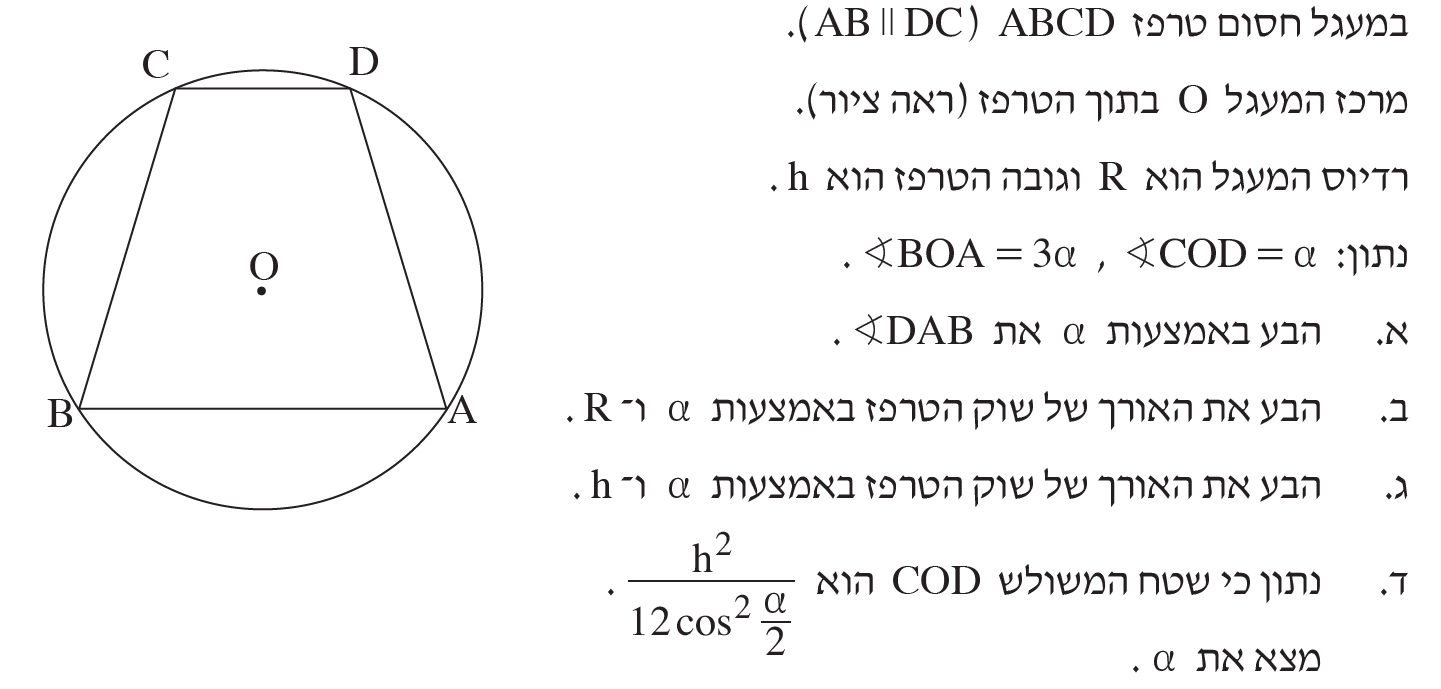
\includegraphics[width=\textwidth]{summer-2016b-5}
\end{center}

\vspace{-2ex}


מהתרשים נראה שהטרפז שווה-שוקיים, אבל אין לסמוך על תרשימים. השקעתי זמן רב עד שעלה בדעתי האפשרות שטרפז חסום במעגל חייב להיות שווה-שוקיים. המשפט לא מופיע ברשימת המשפטים שניתן לצטט בבחינת הבגרות ויש להוכיח אותו. בספרי לימוד המשפט לא מובלט ומופיע רק כדוגמה או תרגיל. אני אביא שתי הוכחות: אחת שלי ואחת המופיעה בספרים.

ההוכחה מהספרים )רשים ימני למטה(:
$\angle ACD = \angle CAB$
לפי זוויות מתחלפות ולכן גם המיתרים הכלואים שווים
$CB=AD$.

ההוכחה שלי )תרשים שמאלי למטה(: המשפט הראשון שחשבתי עליו כאשר קראתי את השאלה הוא משפט 
$56$
"ניתן לחסום מרובע במעגל אם ורק אם סכום זוג זוויות נגדיות שווה ל-%
$180^\circ$".
נסמן
$\angle DAB=\theta$,
ולפי המשפט 
$\angle DCB=180\!-\!\theta$.
לפי זוויות משלימות ומתאימות
$\angle DCF=\angle ABC=\theta$.
לפי משפט
$40$
"טרפז בו הזוויות שליד אותו בסיס שוות זו לזו הוא טרפז שווה שוקיים", הטרפז שווה-שוקיים.

\vspace{-4ex}

\begin{center}
\selectlanguage{english}
\begin{tikzpicture}[scale=.7]
\coordinate (O) at (2,1.5);
\coordinate (B) at (0,.2);
\coordinate (A) at (4,.2);
\node[draw,thick,circle through=(A),name path=circle] at (O) {};
\fill (B) node[left,xshift=-2pt] {$B$} node[above right] {$\theta$?}  circle(1.5pt);
\fill (A) node[right] {$A$} circle(1.5pt);
\path[name path=bc] (B) -- +(75:4);
\path[name path=ad] (A) -- +(105:4);
\path[name intersections={of=bc and circle,by={C}}];
\path[name intersections={of=ad and circle,by={D}}];
\fill (C) node[above left] {$C$} circle(1.5pt);
\fill (D) node[above right] {$D$} circle(1.5pt);
\draw[thick] (B) -- (A) node[above left,xshift=-2pt] {$\theta$} -- (D) -- (C) node[below right,xshift=-2pt] {$180\!-\!\theta$} node[above right,xshift=2pt,yshift=2pt] {$\theta$} -- cycle;
\draw[thick] (B) -- ($(B)!1.3!(C)$) coordinate (F);
\fill (F) node[above right] {$F$} circle(1.5pt);
\end{tikzpicture}
\hspace{4em}
\begin{tikzpicture}[scale=.7]
\coordinate (O) at (2,1.5);
\coordinate (B) at (0,.2);
\coordinate (A) at (4,.2);
\node[draw,thick,circle through=(A),name path=circle] at (O) {};
\fill (B) node[left,xshift=-2pt] {$B$}  circle(1.5pt);
\fill (A) node[right] {$A$} circle(1.5pt);
\path[name path=bc] (B) -- +(75:4);
\path[name path=ad] (A) -- +(105:4);
\path[name intersections={of=bc and circle,by={C}}];
\path[name intersections={of=ad and circle,by={D}}];
\fill (C) node[above left] {$C$} circle(1.5pt);
\fill (D) node[above right] {$D$} circle(1.5pt);
\draw[thick] (B) -- (A) --(D) -- (C) -- cycle;
\draw[thick] (C) node[below right,xshift=10pt] {$\theta$} -- (A) node[above left,xshift=-10pt] {$\theta$};
\end{tikzpicture}
\end{center}

%\np

\textbf{סעיף א}

בארבעת המשולשים עם קודקוד
$O$,
הצלעות המקווקוות הם רדיוסים שאורכם
$R$,
והמשולשים שווה שוקיים.
$\triangle COB\cong \triangle DOA$
לפי צ.צ.צ. כי הטרפז שווה שוקיים. מכאן ש-%
$\angle COB\cong \angle DOA$,
וניתן לסמן את הזוויות לפי החישובים מימין לתרשים. החישוב של
$\gamma$
מוצדק כי סכום הזוויות סביב נקודה הוא 
$360$.
השורה האחרונה מציגה את התשובה לשאלה כי
$\angle DAB=\beta+\delta$.

\np

%\begin{center}
\selectlanguage{english}
\hspace{1em}
\begin{minipage}{.4\textwidth}
\begin{tikzpicture}%[scale=.9]
\coordinate (O) at (2,1.5);
\coordinate (B) at (0,.2);
\coordinate (A) at (4,.2);
\node[draw,thick,circle through=(A),name path=circle] at (O) {};
\fill (O) node[left,xshift=-4pt,yshift=2pt] {$O$} node[below,yshift=-6pt] {$3\alpha$} node[above,yshift=10pt] {$\alpha$} node[right,xshift=6pt] {$\gamma$} circle(1.5pt);
\fill (B) node[left,xshift=-2pt] {$B$} node[above right,xshift=26pt] {$\beta$} circle(1.5pt);
\fill (A) node[right] {$A$} node[above left,xshift=-22pt] {$\beta$} node[above left,xshift=-6pt,yshift=14pt] {$\delta$} circle(1.5pt);
\path[name path=bc] (B) -- +(75:4);
\path[name path=ad] (A) -- +(105:4);
\path[name intersections={of=bc and circle,by={C}}];
\path[name intersections={of=ad and circle,by={D}}];
\fill (C) node[above left] {$C$} circle(1.5pt);
\fill (D) node[above right] {$D$} node[below left,xshift=4pt,yshift=-12pt] {$\delta$}  circle(1.5pt);
\draw[thick] (B) -- (A) --(D) -- (C) -- cycle;
\draw[thick,dashed] (O) -- (A);
\draw[thick,dashed] (O) -- (B);
\draw[thick,dashed] (O) -- (C);
\draw[thick,dashed] (O) -- (D);
\draw[very thick,dotted] (C) -- node[right,yshift=4pt] {$h$} ($(B)!(C)!(A)$) node[below] {$E$};
\draw[rotate=90] ($(B)!(C)!(A)$) rectangle +(6pt,6pt);
\end{tikzpicture}
\end{minipage}
\begin{minipage}{.4\textwidth}
\erh{12pt}
\begin{equationarray*}{rcl}
\beta &=& \frac{180-3\alpha}{2}\\
\gamma &=& \frac{360-(\alpha+3\alpha)}{2}=180-2\alpha\\
\delta &=&\frac{180-\gamma}{2}= \frac{180-(180-2\alpha)}{2}=\alpha\\
\beta+\delta&=&\frac{180-\alpha}{2}\,.
\end{equationarray*}
\end{minipage}
\selectlanguage{hebrew}
%\end{center}

\textbf{סעיף ב}

כדי חשב אורך של שוק נחפש משולש שאחד מצלעותיו הוא
$DA$.
לפי חוק בסינוסים ב-%
$\triangle DOA$:
\erh{12pt}
\begin{equationarray*}{rcl}
\frac{DA}{\sin\gamma}&=&\frac{R}{\sin\delta}\\
\frac{DA}{\sin(180\!-\!2\alpha)}&=&\frac{R}{\sin\alpha}\\
DA&=&\frac{R\sin 2\alpha}{\sin\alpha}\\
&=&\frac{R\cdot 2\sin \alpha\cos\alpha}{\sin\alpha} = 2R\cos\alpha\,.
\end{equationarray*}

\vspace{-4ex}

\textbf{סעיף ג}

בתרשים ציירנו את הגובה מהנקודה 
$C$
כדי לא להסתיר את הסימונים ב-%
$\triangle DOA$.
$CB=DA$
הוא גם שוק. נשתמש בהגדרה של סינוס במשולש 
$\triangle CBE$:
\[
\frac{h}{CB}=\sin \angle CBE=\sin \left(\frac{180\!-\!3\alpha}{2}+\alpha\right)=\sin \left(90-\frac{\alpha}{2}\right)=\cos\frac{\alpha}{2}\,.
\]
כי
$\angle CBE=\angle DAB=\beta+\delta$.
התשובה היא
$CB=\displaystyle\frac{h}{\cos (\alpha/2)}$.

\textbf{סעיף ד}

בנוסחה הטריגונטמרית עבור
$S_{\triangle COD}$
יופיעו אורכי הצלעות
$R$
והזווית
$\alpha$.
אנו רוצים נוסחה עם 
$h$
ו-%
$\alpha$
כדי להשוות לביטוי הנתון. נשווה את הביטויים עבור שוקי הטרפז מהסעיפים הקודמים:
\erh{12pt}
\begin{equationarray*}{rcl}
2R\cos\alpha&=&\frac{h}{\cos(\alpha/2)}\\
R&=&\frac{h}{2\cos\alpha \cos(\alpha/2)}\,.
\end{equationarray*}

\np

נציב בנוסחה לשטח, נשווה לנוסחה הנתונה לשטח ונצמצם:
\erh{16pt}
\begin{equationarray*}{rcl}
S_{\triangle COD}&=&\frac{1}{2}\cdot OC \cdot OD \cdot \sin\alpha=\frac{1}{2}R^2\sin\alpha\\
&=&\frac{1}{2}\cdot \frac{h^2}{4}\cdot \frac{1}{\left(\cos\alpha \cos(\alpha/2)\right)^2} \cdot \sin\alpha\\
\frac{h^2}{12\cos^2 (\alpha/2)}&=&\frac{1}{2}\cdot \frac{h^2}{4}\cdot \frac{1}{\left(\cos\alpha \cos(\alpha/2)\right)^2} \cdot \sin\alpha\\
\frac{1}{12}&=&\frac{1}{8}\cdot \frac{1}{\cos^2\alpha} \cdot \sin\alpha\\
\frac{1}{12}&=&\frac{1}{8}\cdot \frac{1}{1-\sin^2\alpha} \cdot \sin\alpha\,.
\end{equationarray*}
נקבל משוואה ריבועית ב-%
$\sin\alpha$,
ונבחר את השורש 
$\displaystyle\frac{1}{2}$
כי הערך של סינוס לא יכול להיות
$-2$:
\erh{12pt}
\begin{equationarray*}{rcl}
2\sin^2\alpha + 3\sin\alpha - 2&=&0\\
(2\sin\alpha-1)(\sin\alpha+2)&=& 0\\
\sin\alpha&=&\frac{1}{2}\,.
\end{equationarray*}
הערך היחיד ש-%
$\alpha$
יכול לקבל הוא
$30^\circ$
כי זוויות הבסיס של טרפז חייבים להיות פחות מ-%
$90^\circ$.

%%%%%%%%%%%%%%%%%%%%%%%%%%%%%%%%%%%%%%%%%%%%%%%%%%%%%%%%%%%%%%


\np

\section{קיץ תשע"ו מועד א}

\begin{center}
\selectlanguage{english}
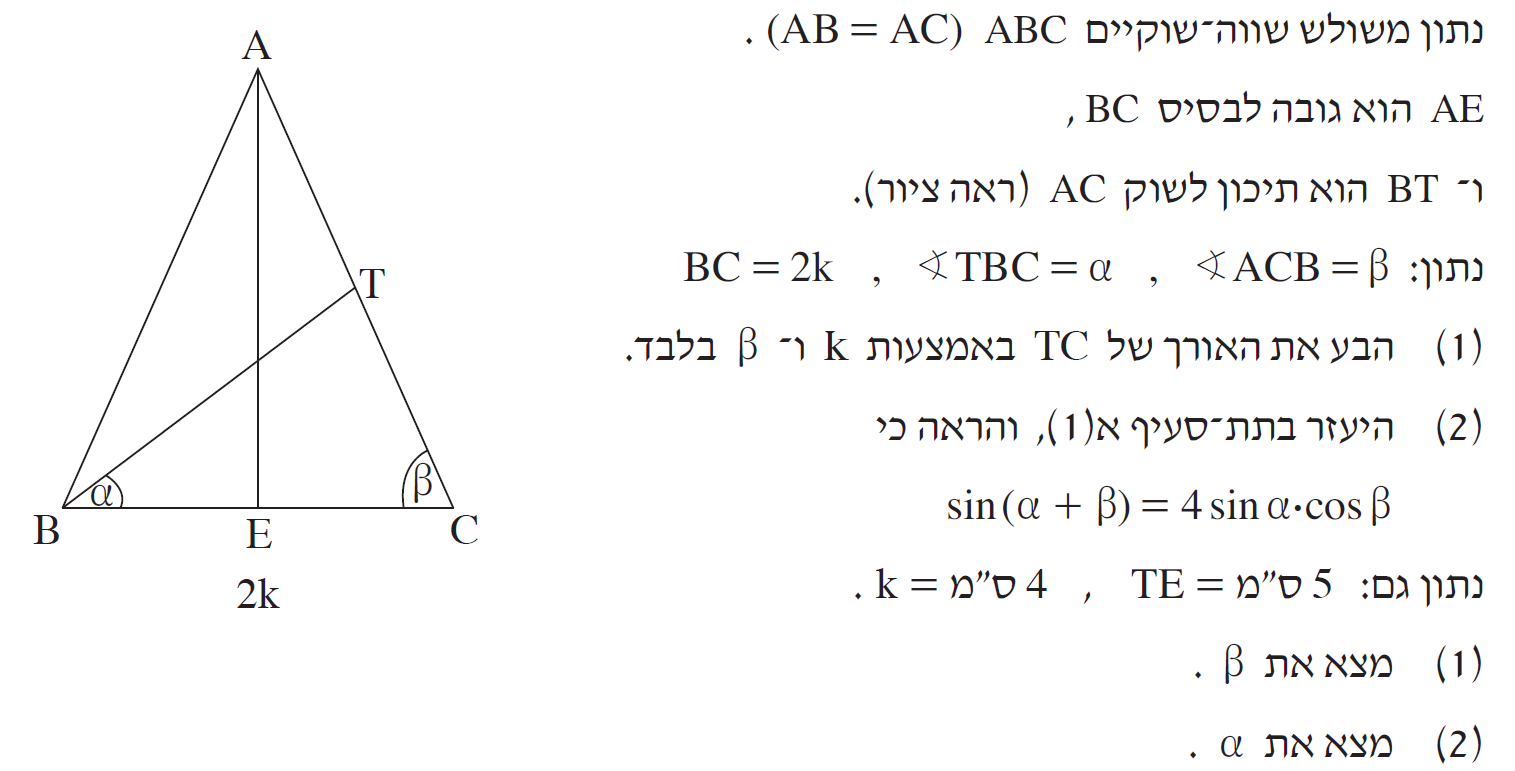
\includegraphics[width=\textwidth]{summer-2016a-5}
\end{center}

\vspace{-3ex}

\begin{center}
\selectlanguage{english}
\begin{tikzpicture}[scale=.85]
\coordinate (B) at (0,0);
\coordinate (C) at (5,0);
\path[name path=ba] (B) -- +(66:7);
\path[name path=ca] (C) -- +(114:7);
\path[name intersections={of=ba and ca,by={A}}];
\fill (A) node[above] {$A$} circle(1.5pt);
\fill (B) node[below left] {$B$} node[above right,xshift=12pt] {$\alpha$} circle(1.5pt);
\fill (C) node[below right] {$C$} node[above left,xshift=-6pt] {$\beta$} circle(1.5pt);
\coordinate (T) at ($(A)!.5!(C)$);
\fill (T) node[right] {$T$} circle(1.5pt);
\draw[thick] (B) -- (T);
\coordinate (E) at ($(B)!(A)!(C)$);
\draw[thick] (A) -- (E);
\fill (E) node[below] {$E$} circle(1.5pt);
\draw[rotate=90] (E) rectangle +(8pt,8pt);
\draw[thick] (A) -- node[left] {$2a$} (B) -- node[below] {$k$} (E) -- node[below] {$k$} (C) -- node[right] {$a$} (T) -- node[right] {$a$} (A);
\node at ($(T)+(60pt,-10pt)$) {$180\!-\!(\alpha\!+\!\beta)$};
\draw[->] ($(T)+(25pt,-9pt)$) -- +(-28pt,0);
\end{tikzpicture}
\end{center}

\vspace{-1ex}

$\bm{(1)}$
לפי הגדרת קוסינוסים ב-%
$\triangle AEC$:

\vspace{-3ex}

\erh{12pt}
\begin{equationarray*}{rcl}
\cos \beta &=& \frac{k}{2a}\\
TC = a &=& \frac{k}{2\cos\beta}\,.
\end{equationarray*}

\vspace{-2ex}

$\bm{(2)}$
נחפש משולש עבורו חוק הסינוסים ייתן משוואה בה יצטמצם
$k$
או
$a$.
$\triangle TBC$ 
מתאים:

\vspace{-5ex}

\selectlanguage{english}
\erh{14pt}
\begin{equationarray*}{rcl}
\frac{2k}{\sin(180\!-\!(\alpha\!+\!\beta))}&=&\frac{a}{\sin\alpha}\\
\frac{2k}{\sin(\alpha\!+\!\beta)}&=&\frac{k/(2\cos\beta)}{\sin\alpha}\\
\sin(\alpha\!+\!\beta)&=&4\sin\alpha\cos\beta\,.
\end{equationarray*}
\selectlanguage{hebrew}

\np

$\bm{(1)}$
נוסיף את אורכי הצלעות הנתונים ונשתמש במשפט
$86$
"במשולש ישר זווית התיכון ליתר שווה למחצית היתר" כדי להסיק ש-%
$TE=TA=TC=5$
ו-%
$\triangle ETC$
שווה-שוקיים:
\begin{center}
\selectlanguage{english}
\begin{tikzpicture}[scale=.9]
\coordinate (B) at (0,0);
\coordinate (C) at (5,0);
\path[name path=ba] (B) -- +(66:7);
\path[name path=ca] (C) -- +(114:7);
\path[name intersections={of=ba and ca,by={A}}];
\fill (A) node[above] {$A$} circle(1.5pt);
\fill (B) node[below left] {$B$} node[above right,xshift=12pt] {$\alpha$} circle(1.5pt);
\fill (C) node[below right] {$C$} node[above left,xshift=-6pt] {$\beta$} circle(1.5pt);
\coordinate (T) at ($(A)!.5!(C)$);
\fill (T) node[right] {$T$} circle(1.5pt);
\draw[thick] (B) -- (T);
\coordinate (E) at ($(B)!(A)!(C)$);
\draw[thick] (A) -- (E);
\fill (E) node[below] {$E$} node[above right,xshift=2pt] {$\beta$}circle(1.5pt);
\draw[rotate=90] (E) rectangle +(8pt,8pt);
\draw[thick] (A) -- (B) -- (C) -- node[right] {$5$} (T) -- node[right] {$5$} (A);
\coordinate (F) at ($(E)!(T)!(C)$);
\draw[thick,dashed] (E) -- node[above,xshift=-2pt] {$5$} (T) -- (F);
\path (B) -- node[below] {$4$} (E) -- node[below] {$2$} (F) -- node[below] {$2$} (C);
\draw (F) rectangle +(8pt,8pt);
\end{tikzpicture}
\end{center}

נוריד גובה מ-%
$T$
שהוא אנך אמצעי במשלוש שווה-שוקיים
$\triangle ETC$
ונקבל:
\erh{10pt}
\begin{equationarray*}{rcl}
\cos\beta &=& \frac{2}{5}\\
\beta &=&66.4^\circ\,.
\end{equationarray*}

\vspace{-4ex}

$\bm{(2)}$
לפי סעיף 
$(1)$
וסעיף 
$(2)$
הקודם:

\vspace{-5ex}

\erh{14pt}
\begin{equationarray*}{rcl}
\sin(\alpha+\beta)&=&4\sin\alpha\cos\beta\\
\sin\alpha\cos\beta+\cos\alpha\sin\beta&=&4\sin\alpha\cos\beta\\
\sin\alpha\cdot\frac{2}{5}+\cos\alpha\sqrt{1-\left(\frac{2}{5}\right)^2}&=&4\sin\alpha\cdot\frac{2}{5}\\
\sqrt{21}\cos\alpha&=&6\sin\alpha\\
\tan\alpha &=& \frac{\sqrt{21}}{6}\\
\alpha&=&37.37^\circ\,.
\end{equationarray*}

%%%%%%%%%%%%%%%%%%%%%%%%%%%%%%%%%%%%%%%%%%%%%%%%%%%%%%%%%%%%%%
\np


\section{חורף תשע"ו}

\begin{center}
\selectlanguage{english}
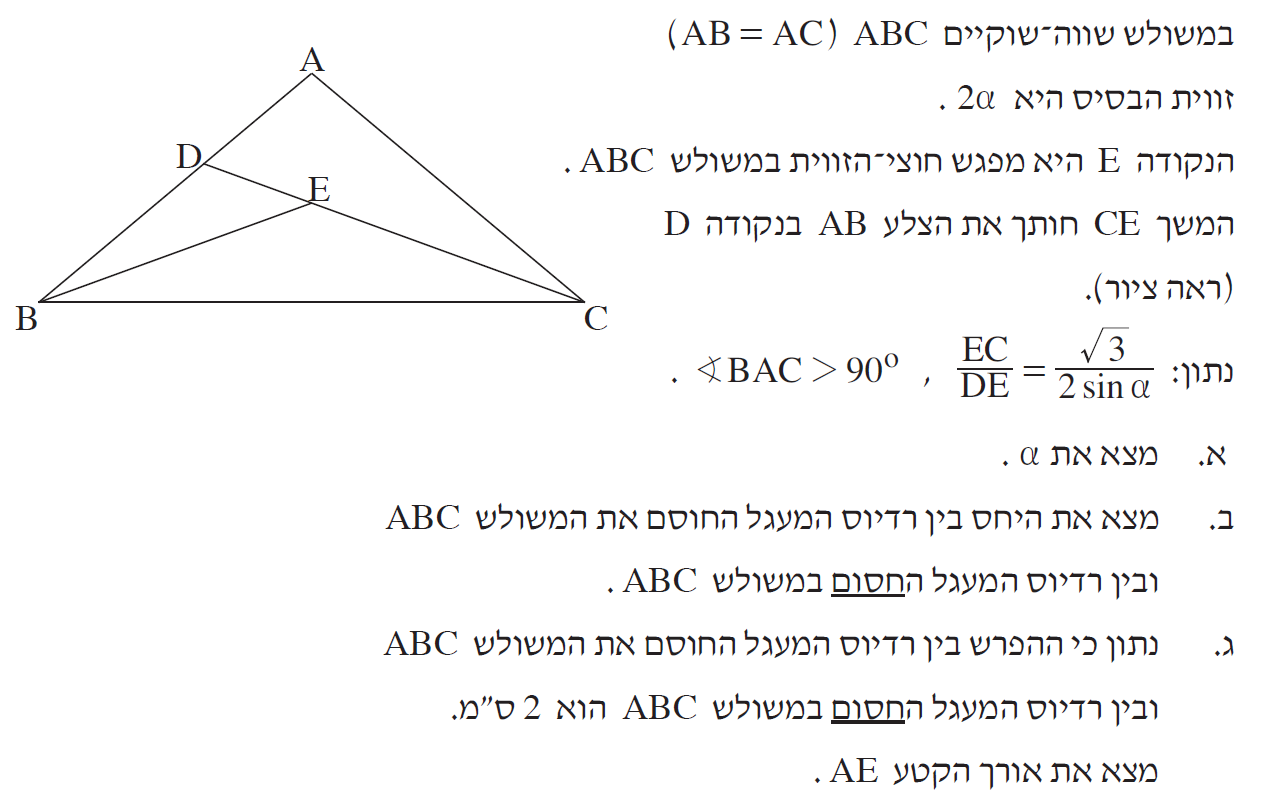
\includegraphics[width=\textwidth]{winter-2016-5}
\end{center}

נתון שהנקודה 
$E$
היא מפגש חוצי הזוויות. לפי משפט
$6$
"במשולש שווה שוקיים , חוצה זווית הראש, התיכון לבסיס והגובה לבסיס מתלכדים", ולכן חוצה הזווית
$\angle A$
עובר דרך
$E$
וחותך את
$BC$
בנקודה 
$F$
בזווית ישרה. נסמן כמה זוויות שאפשר תוך שימוש רק במשפטים פשוטים כגון סכום הזוויות במשולש הוא
$180$.
$\triangle EFB\cong \triangle EFC$
לפי צ.ז.צ. )%
$F$
היא נקודת האמצע של
$BC$,
זוויות ב-%
$F$
ישרות ושוות,
$EF$
צלע משותף(. לכן, הזוויות 
$\angle BEF=\angle CEF=90\!-\!\alpha$
שנסמן 
$\beta$.
בדרך דומה אפשר להסיק ש-%
$\angle BAF=\angle CAF=90\!-\!2\alpha$
שנסמן
$\gamma$.
$\angle AED=\beta$
לפי זוויות קודקודיות, ו:
\[
\angle ADE=180-\beta-\gamma=180-(90\!-\!\alpha)-(90\!-\!2\alpha)=3\alpha\,.
\]
לבסוף 
$\angle BDE=180\!-\!3\alpha$
לפי זוויות משלימות.
\begin{center}
\selectlanguage{english}
\begin{tikzpicture}%[scale=1.1]
\coordinate (B) at (0,0);
\coordinate (C) at (10,0);
\path[name path=ba] (B) -- +(40:7);
\path[name path=ca] (C) -- +(140:7);
\path[name intersections={of=ba and ca,by={A}}];
\fill (A) node[above] {$A$} node[below right,xshift=0pt,yshift=-8pt] {$\gamma$} node[below left,yshift=-8pt] {$\gamma$} circle(1.5pt);
\fill (B) node[below left] {$B$} node[above right,xshift=24pt,yshift=12pt] {$\alpha$} node[above right,xshift=30pt] {$\alpha$} circle(1.5pt);
\fill (C) node[below right] {$C$} node[above left,xshift=-24pt,yshift=12pt] {$\alpha$} node[above left,xshift=-30pt] {$\alpha$} circle(1.5pt);
\draw[thick] (A) -- (B) -- (C) -- cycle;
\path[name path=cbis] (C) -- +(160:8);
\path[name path=bbis] (B) -- +(20:8);
\path[name intersections={of=ba and cbis,by={D}}];
\path[name intersections={of=bbis and cbis,by={E}}];
\fill (D) node[left] {$D$} node[right,xshift=8pt,yshift=2pt] {$3\alpha$} node[below left,xshift=-20pt] {$180\!-\!3\alpha$} circle(1.5pt);
\draw[->] ($(D)+(-22pt,-10pt)$) -- +(20pt,0);
\fill (E) node[above right] {$E$} node[above left,yshift=2pt] {$\beta$} node[below left,yshift=-4pt] {$\beta$} node[below right,yshift=-4pt] {$\beta$} node[left,xshift=-10pt] {$2\alpha$} circle(1.5pt);
\draw[thick] (C) -- (D);
\draw[thick] (B) -- node[above] {$a$} (E);
\path (C) -- node[above] {$a$} (E);
\coordinate (F) at (A |- B);
\draw[thick,dashed] (A) -- (F);
\fill (F) node[below] {$F$} circle(1.5pt);
\draw (F) rectangle +(8pt,8pt);
\node at ($(A)+(80pt,-10pt)$) {$\beta = 90\!-\!\alpha$};
\node at ($(A)+(83pt,-26pt)$) {$\gamma = 90\!-\!2\alpha$};
\path (E) -- node[right,yshift=-4pt] {$r$} (F);
\end{tikzpicture}
\end{center}

\np

\textbf{סעיף א}

נתון היחס 
$\frac{EC}{DE}$
כתלות ב-%
$\alpha$,
ולכן נחפש מקרה של חוק הסינוסים שייתן אל היחס בדרך אחרת עם
$\alpha$.
אמנם 
$EC,DE$
הם צלעות במשולשים שונים, אבל כבר הוכחנו ש-%
$\triangle EFB\cong \triangle EFC$
כך ש-%
$EB=EC$.
לפי חוק הסינוסים:
\erh{14pt}
\begin{equationarray*}{rcl}
\frac{EB}{\sin(180\!-\!3\alpha)}&=&\frac{DE}{\sin\alpha}\\
\frac{EB}{DE}&=&\frac{\sin(180\!-\!3\alpha)}{\sin\alpha}=\frac{\sin 3\alpha}{\sin\alpha}\\
\frac{\sqrt{3}}{2\sin\alpha}&=&\frac{\sin3\alpha}{\sin\alpha}\\
\sin 3\alpha&=&\frac{\sqrt{3}}{2}\,.
\end{equationarray*}
מכאן ש-%
$\alpha=20^\circ$.

\textbf{סעיף ב}

לפי משפט
$49$
"שלושת חוצי הזוויות של משולש נחתכים בנקודה אחת, שהיא מרכז המעגל החסום במשולש", הנקודה
$E$
היא מרכז המעגל החסום שמשיק לצלעות. נקודת ההשקה ניצב לרדיוס ולכן המעגל משיק למשולש בנקודה
$F$.
מכאן ש-%
$EF$
הוא הרדיוס של המעגל החסום וסימנו אותו
$r$.

כעת צריך להימנע מהפיתוי לקבוע ש-%
$E$
היא גם מרכזו של המעגל החוסם. אמנם
$AF$
הוא האנך האמצעי ל-%
$BC$,
אבל אנחנו לא יודעים דבר על האנכים האמצעיים של הצלעות האחרים.

במקום זה נשתמש בחוק הסינוסים על
\textbf{המשלוש}
$\bm{\triangle ABC}$.
נבחר את הזווית
$\angle BAC$
והצלע
$BC$
כי אנו יודעים לחשב את אורך הצלע כתלות ב-%
$r,\alpha$:

\vspace{-6ex}
\erh{14pt}
\begin{equationarray*}{rcl}
BC&=&2BF=\frac{2r}{\tan \alpha}\\
2R&=&\frac{BC}{\sin (180\!-\!4\alpha)}=\frac{BC}{\sin 4\alpha}\\
\frac{R}{r}&=&\frac{1}{\sin 4\alpha\cdot\tan \alpha}=\frac{1}{\sin 80\cdot\tan 20}=2.79\,.
\end{equationarray*}

\vspace{-2ex}

\textbf{סעיף ג}

נתון
$R-r=2$,
ולכן
$r=2/(2.79-1)=1.117$.
אין לנו הרבה מידע על המשולשים
$\triangle AED,\triangle AEC$,
כך שנראה שהדרך לחשב את
$AE$
היא לחשב את 
$AF$
ולהחסיר
$EF=r$:
\erh{14pt}
\begin{equationarray*}{rcl}
\tan 2\alpha&=&\frac{AE+r}{BC/2}=\frac{(AE+r)\tan\alpha}{r}\\
AE&=&\frac{r(\tan 2\alpha - \tan \alpha)}{\tan \alpha}=1.117\cdot \frac{\tan 40-\tan 20}{\tan 20}\\
&=&1.117\cdot \frac{0.839-0.3640}{0.3640}=1.458\,.
\end{equationarray*}

%%%%%%%%%%%%%%%%%%%%%%%%%%%%%%%%%%%%%%%%%%%%%%%%%%%%%%%%%%%%%%


\np

\section{קיץ תשע"ה מועד ב}

\begin{center}
\selectlanguage{english}
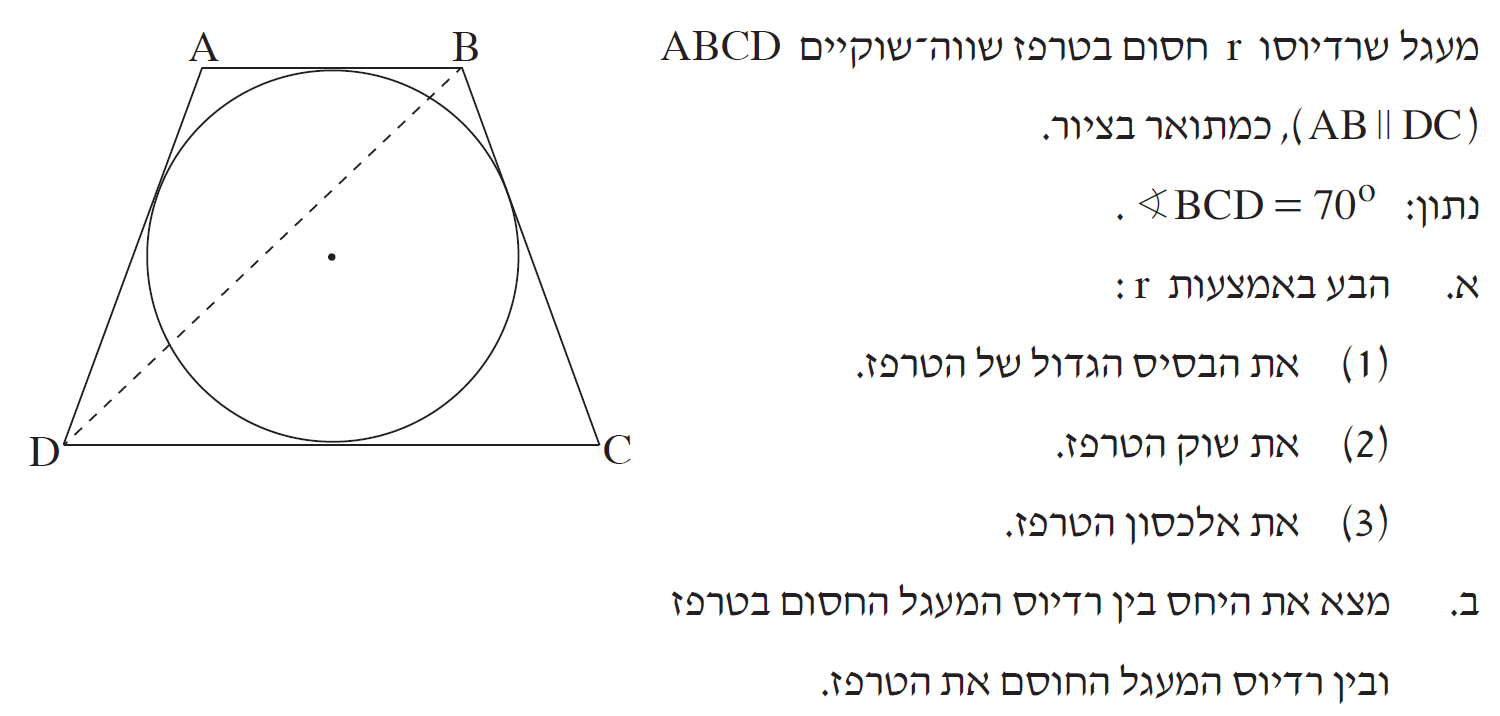
\includegraphics[width=\textwidth]{summer-2015b-5}
\end{center}

\vspace{-1ex}

\textbf{סעיף א}

הוספנו סימונים לתרשים ונצטרך להצדיק אותם. 
משפט
$77$
"המשיק למעגל מאונך לרדיוס בנקודת ההשקה" ולכן הקו 
$EF$
הניצב לצלעות המקיבלים 
$AB\|DC$
הוא באורך
$2r$.
$AG, BH$
אנכים מ-%
$AB$ 
ל-%
$DC$,
כך ש-%
$AG=EF=BF=2r$,
ו-%
$AB=GH=b_2$.
הטרפז שווה-שוקיים ולפי משפט
$39$
"בטרפז שווה שוקיים הזוויות שליד אותו בסיס שוות זו לזו", 
$\angle ADC=\angle BCD=70^\circ$.

\begin{center}
\selectlanguage{english}
\begin{tikzpicture}[scale=1.1]
\node[circle,draw,thick] (In) at (0,0) [minimum size=5.45cm] {};
\fill (In) circle(1.5pt);
\coordinate (D) at (-3.5,-2.5);
\draw[thick] (D) -- +(7,0) coordinate (C) node[above left,xshift=-2pt] {$70$};
\fill (C) node[below right] {$C$} circle(1.5pt);
\fill (D) node[below left] {$D$}  node[above right,xshift=2pt] {$70$} circle(1.5pt);
\coordinate (DA) at (tangent cs:node=In,point={(D)},solution=2);
\path[name path=da] (D) -- ($(D)!1.7!(DA)$);
\fill (DA) circle(1.5pt);
\coordinate (CB) at (tangent cs:node=In,point={(C)},solution=1);
\path[name path=cb] (C) -- ($(C)!1.7!(CB)$);
\fill (CB) circle(1.5pt);
\path[name path=top] (-3,2.5) -- (3,2.5);
\path[name intersections={of=da and top,by={A}}];
\path[name intersections={of=cb and top,by={B}}];
\fill (A) node[above left] {$A$} circle(1.5pt);
\fill (B) node[above right] {$B$} circle(1.5pt);
\draw[thick] (D) -- node[left] {$s$} (A) -- (B) -- node[right] {$s$} (C);
\draw[thick,dashed] (D) -- (B);
\coordinate (AB) at (0,2.5);
\fill (AB)  node[above] {$E$} circle (1.5pt);
\coordinate (DC) at (0,-2.5);
\fill (DC)  node[below,yshift=-1pt] {$F$} circle (1.5pt);
\draw[thick,dashed] (AB) -- node[left,yshift=-6pt] {$2r$} (DC);
\coordinate (ADC) at ($(D)!(A)!(C)$);
\draw[thick,dashed] (A) -- node[right,yshift=8pt] {$2r$} (ADC);
\fill (ADC) node[below,yshift=-1pt] {$G$} circle(1.5pt);
\coordinate (BDC) at ($(D)!(B)!(C)$);
\draw[thick,dashed] (B) -- node[left,yshift=8pt] {$2r$} (BDC);
\fill (BDC) node[below,yshift=-1pt] {$H$} circle(1.5pt);
\draw (ADC) rectangle +(8pt,8pt);
\draw (BDC) rectangle +(8pt,8pt);
\draw (DC) rectangle +(8pt,8pt);
\draw[<->] ($(D)+(0,-8mm)$) -- node[fill=white] {$b_1$} ($(ADC)+(0,-8mm)$);
\draw[<->] ($(ADC)+(0,-8mm)$) -- node[fill=white] {$b_2$} ($(BDC)+(0,-8mm)$);
\draw[<->] ($(BDC)+(0,-8mm)$) -- node[fill=white] {$b_1$} ($(C)+(0,-8mm)$);
\draw[<->] ($(D)+(0,-14mm)$) -- node[fill=white] {$b$} ($(C)+(0,-14mm)$);
\draw[<->] ($(A)+(0,8mm)$) -- node[fill=white] {$b_2$} ($(B)+(0,8mm)$);
\end{tikzpicture}
\end{center}

\np

$\triangle ADG \cong \triangle BCH$
לפי ז.צ.ז: מהשלמת הזוויות במשולשים,
$\angle DAG=\angle CBH=180-90-70$.
מכאן ש-%
$DG=HC=b_1$,
והבסיס הוא
$b=2b_1+b_2$.

כעת נוכל לגשת לחישוב הערכים המבוקשים בסעיף.


$(1)$
לפי משפט
$57$
"מרובע קמור חוסם מעגל אם ורק אם סכום שתי צלעות נגדיות שווה לסכום שתי הצלעות הנגדיות האחרות":
\vspace{-6ex}

\erh{12pt}
\begin{equationarray*}{rcl}
2s&=&b_2+(b_1+b_2+b_1)\\
b_2 &=&s-b_1\\
\tan 70 &=& \frac{2r}{b_1}\\
\sin 70&=&\frac{2r}{s}\\
b&=&2b_1+b_2=2b_1+(s-b_1)=b_1+s\\
&=&2r\left(\frac{1}{\tan 70}+\frac{1}{\sin 70}\right)\\
&=&2.856r\,.
\end{equationarray*}

\vspace{-3ex}

$(2)$
$s=\displaystyle\frac{2r}{\sin 70}=2.128r$.

\medskip

$(3)$
האלכסון הוא היתר של 
$\triangle BDH$
שצלעותיו ידועים:

\vspace{-6ex}

\erh{18pt}
\begin{equationarray*}{rcl}
DB^2&=& (b_1+b_2)^2 + (2r)^2\\
&=&s^2 +(2r)^2\\
&=& \left(\frac{2r}{\sin 70}\right)^2 + 4r^2\\
DB&=&2r\sqrt{\left(\frac{1}{\sin 70}\right)^2+1}\\
&=&2.921r\,.
\end{equationarray*}

\vspace{-3ex}

\textbf{סעיף ב}

במבט ראשון נראה שכדאי להשתמש במשפט
$56$
"ניתן לחסום מרובע במעגל אם ורק אם סכום זוג זוויות נגדיות שווה ל-%
$180^\circ$",
אבל יש לנו כל כך הרבה מידע על הטרפז שאין בו צורך.


\textbf{שימו לב!!}
המרכז של המעגל החוסם
$M_1$
אינו בהכרח המרכז של המעגל החסום
$M_2$.
ניסיתי לחשב את 
$R$
לפי פיתגורס ב-%
$\triangle FM_2C$
אבל זה לא נכון.

\np

\begin{center}
\selectlanguage{english}
\begin{tikzpicture}[scale=1.1]
\node[circle,draw,thick] (In) at (0,0) [minimum size=5.45cm] {};
\fill (In) circle(1.5pt);
\coordinate (D) at (-3.5,-2.5);
\draw[thick] (D) -- +(7,0) coordinate (C) node[above left,xshift=-2pt] {$70$};
\fill (C) node[below right] {$C$} circle(1.5pt);
\fill (D) node[below left] {$D$} circle(1.5pt);
\coordinate (DA) at (tangent cs:node=In,point={(D)},solution=2);
\path[name path=da] (D) -- ($(D)!1.7!(DA)$);
%\fill (DA) circle(1.5pt);
\coordinate (CB) at (tangent cs:node=In,point={(C)},solution=1);
\path[name path=cb] (C) -- ($(C)!1.7!(CB)$);
%\fill (CB) circle(1.5pt);
\path[name path=top] (-3,2.5) -- (3,2.5);
\path[name intersections={of=da and top,by={A}}];
\path[name intersections={of=cb and top,by={B}}];
\fill (A) node[above left] {$A$} circle(1.5pt);
\fill (B) node[above right] {$B$} circle(1.5pt);
\draw[thick] (D) -- (A) -- (B) -- (C);
\draw[ultra thick] (D) -- (B) -- (C) -- cycle;
\coordinate (AB) at (0,2.5);
\coordinate (DC) at (0,-2.5);
\fill (DC)  node[below,yshift=-1pt] {$F$} circle (1.5pt);
\coordinate (ADC) at ($(D)!(A)!(C)$);
%\draw[thick,dashed] (A) -- node[right,yshift=8pt] {$2r$} (ADC);
%\fill (ADC) node[below,yshift=-1pt] {$G$} circle(1.5pt);
\coordinate (BDC) at ($(D)!(B)!(C)$);
\draw[thick,dashed] (B) -- node[left,yshift=8pt] {$2r$} (BDC);
\fill (BDC) node[below,yshift=-1pt] {$H$} circle(1.5pt);
\draw (BDC) rectangle +(8pt,8pt);
\draw[<->] ($(D)+(0,-8mm)$) -- node[fill=white] {$b_1$} ($(ADC)+(0,-8mm)$);
\draw[<->] ($(ADC)+(0,-8mm)$) -- node[fill=white] {$b_2$} ($(BDC)+(0,-8mm)$);
\tkzCircumCenter(B,D,C)\tkzGetPoint{Cir}
\tkzDrawCircle[thick,dotted,name path=circle](Cir,D)
\fill (Cir) node[right,xshift=2pt,yshift=2pt] {$M_{1}$} circle(1.5pt);
\fill (In) node[above]  {$M_{2}$} circle(1.5pt);
\draw[thick,dotted] (Cir) -- (A);
\draw[thick,dotted] (Cir) -- (B);
\draw[thick,dotted] (Cir) -- (C);
\draw[thick,dotted] (Cir) -- (D);
\end{tikzpicture}
\end{center}
במקום זה יש להשתמש בחוק הסינוסים במשולש
$\triangle BCD$ 
)מודגש(:
\erh{16pt}
\begin{equationarray*}{rcl}
2R&=&\frac{DB}{\sin BCD}=\frac{2.921r}{\sin 70}\\
\frac{r}{R}&=&\frac{2\cdot \sin 70}{2.921}\\
&=&6.434\,.
\end{equationarray*}


%%%%%%%%%%%%%%%%%%%%%%%%%%%%%%%%%%%%%%%%%%%%%%%%%%%%%%%%%%%%%%

\np

\section{קיץ תשע"ה מועד א}

\begin{center}
\selectlanguage{english}
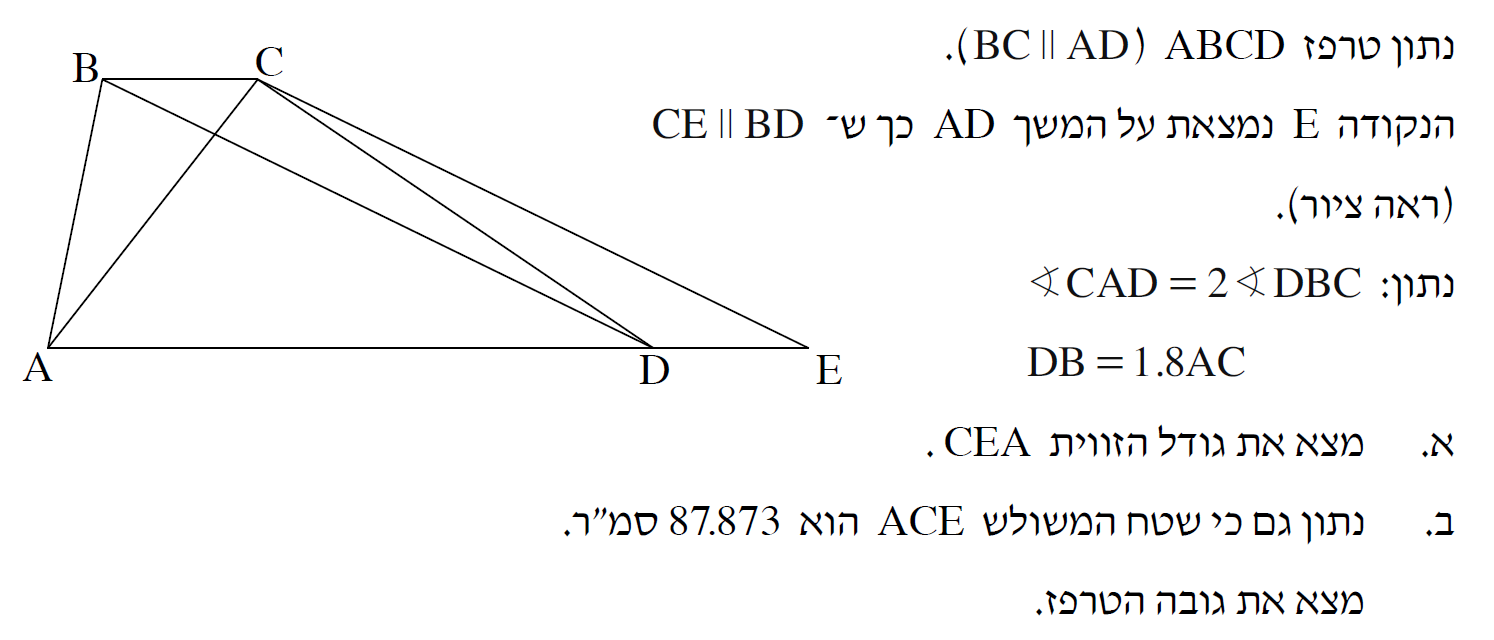
\includegraphics[width=\textwidth]{summer-2015a-5}
\end{center}

\vspace{-1ex}

\textbf{סעיף א}

נסמן בתרשים צלעות וזוויות גם לפי זוויות מתחלפות ומתאימות:
\begin{center}
\selectlanguage{english}
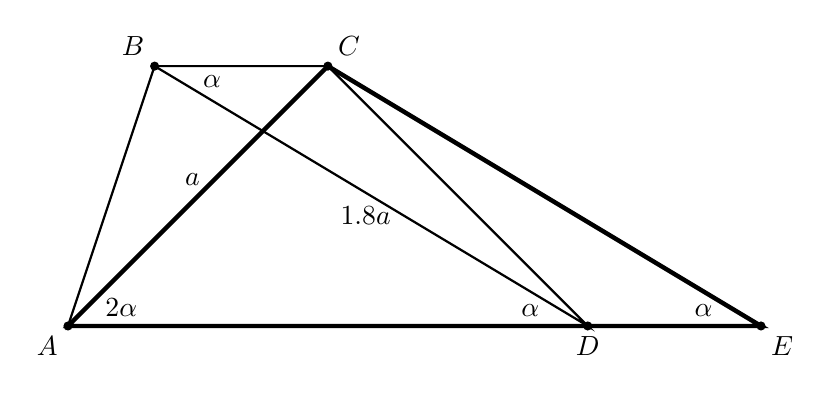
\begin{tikzpicture}[scale=1.1]
\draw[thick] (0,0) coordinate (A) node[below left] {$A$} -- (6,0) coordinate (D) node[below] {$D$} -- (8,0) coordinate (E) node[below right] {$E$} -- (3,3) coordinate (C) node[above right] {$C$} -- (1,3) coordinate (B) node[above left] {$B$} -- (A) -- node[above,xshift=-2pt] {$a$} (C);
\draw[thick] (B) -- node[below,xshift=-2pt] {$1.8a$} (D) -- (C);
\fill (A) node[above right,xshift=10pt] {$2\alpha$} circle(1.5pt);
\fill (B) node[below right,xshift=14pt] {$\alpha$} circle(1.5pt);
\fill (C) circle(1.5pt);
\fill (D) node[above left,xshift=-14pt] {$\alpha$} circle(1.5pt);
\fill (E) node[above left,xshift=-14pt] {$\alpha$} circle(1.5pt);
\draw[ultra thick] (A) -- (E) -- (C) -- cycle;
\end{tikzpicture}
\end{center}

\vspace{-1ex}

כדי לחשב את הזווית 
$\angle CEA=\alpha$
נחפש משלוש שם שני צלעות באורך
$a,1.8a$,
כדי להשתמש בחוק הסינוסים כך שהנעלם
$a$
יצטמצם. אמנם שני הקווים 
$AC,BD$
אינם צלעות של משולש, אבל ניתן לראות ש-%
$BD=CD=1.8a$.
נתון 
$BC\|AD,\,CE\|BD$,
וניתן למשתמש במשפט
$29$
"מרובע שבו כל זוג זוויות נגדיות שוות הוא מקבילית" בגלל זוויות מתחלפות ומתאימות
$\angle CBE,=\angle BDA=\angle CEA=\alpha$,
וזוויות פנימיות
$\angle BCE=\angle BDE=180-\alpha$.

בחוק הסינוסים במשולש המודגש
$ACE$:
\erh{6pt}
\begin{equationarray*}{rcl}
\frac{1}{\sin \alpha} &=& \frac{1.8a}{\sin 2\alpha}\\
1.8\sin \alpha &=& \sin 2\alpha = 2\sin \alpha \cos \alpha\\
\cos \alpha &=& 0.9\\
\alpha &\approx& 25.84\,.
\end{equationarray*}

\np

\textbf{סעיף ב}
נרשום את כל הזוויות במשולש 
$ACE$:
\begin{eqnarray*}
\angle CEA=\alpha &\approx& 25.84\\
\angle CAE=2\alpha &\approx& 51.68\\
\angle ACE=180-3\alpha &\approx& 102.48\,.
\end{eqnarray*}
מהתרשים אפשר לראות ששטח המשולש
$ACE$
מורכב מהשטו של שני משולשים עם אותו גובה:
\begin{center}
\selectlanguage{english}
\begin{tikzpicture}[scale=1.1]
\draw[thick] (0,0) coordinate (A) node[below left] {$A$} -- 
%(6,0) coordinate (D) node[below] {$D$} -- 
(8,0) coordinate (E) node[below right] {$E$} -- (3,3) coordinate (C) node[above right] {$C$} -- (1,3) coordinate (B) node[above left] {$B$} -- (A) -- node[above,xshift=-2pt] {$a$} (C);
%\draw[thick] (B) -- node[below,xshift=-2pt] {$1.8a$} (D) -- (C);
\fill (A) node[above right,xshift=10pt] {$2\alpha$} circle(1.5pt);
\fill (B) circle(1.5pt);
%\fill (B) node[below right,xshift=14pt] {$\alpha$} circle(1.5pt);
\fill (C) circle(1.5pt);
%\fill (D) circle(1.5pt);
%\fill (D) node[above left,xshift=-14pt] {$\alpha$} circle(1.5pt);
\fill (E) node[above left,xshift=-14pt] {$\alpha$} circle(1.5pt);
\draw[ultra thick] (A) -- (E) -- node[right,xshift=2pt,yshift=2pt] {$1.8a$} (C) -- cycle;
\coordinate (F) at ($(A)!(C)!(E)$);
\draw[thick,dashed] (C) -- node[left] {$h$} (F);%($(A)!(C)!(E)$);
\fill (F) circle(1.5pt);
\draw (F) rectangle +(8pt,8pt);
\path (A) -- node[below] {$b_1$} (F) -- node[below] {$b_2$} (E);
\end{tikzpicture}
\end{center}

\vspace{-6ex}

\erh{10pt}
\begin{equationarray*}{rcl}
S_{ACE} &=& \frac{1}{2}(b_1+b_2)h\\
\tan 2\alpha &=& \frac{h}{b_1}\\
\tan \alpha &=& \frac{h}{b_2}\\
S_{ACE} &=& \frac{1}{2}h^2\left(\frac{1}{\tan 2\alpha}+\frac{1}{\tan \alpha}\right)\\
87.873 &=& \frac{1}{2}h^2(6.79+2.06)\\
&=& h^2\cdot 1.425\\
h&\approx& 7.825\,.
\end{equationarray*}
פתרון אחר היא להשתמש בנוסחה לשטח )ששכחתי 
$\ldots$(
שיש לה גורם של סינוס:
\erh{10pt}
\begin{equationarray*}{rcl}
S_{ACE} &=& \frac{1}{2}\cdot AC \cdot CE \cdot \sin ACE\\
&=& \frac{1}{2}\cdot a \cdot 1.8a \cdot \sin (180-3\alpha)\\
87.873 &=& 0.87873 a^2\\
a&=&10\\
h &=& a\sin 2\alpha \approx 7.846\,.
\end{equationarray*}
פתרון זה מעט יותר פשוט ומומלץ למי שלא שכח את הנוסחה.

%%%%%%%%%%%%%%%%%%%%%%%%%%%%%%%%%%%%%%%%%%%%%%%%%%%%%%%%%%%%%%


\np


\section{חורף תשע"ה}

\begin{center}
\selectlanguage{english}
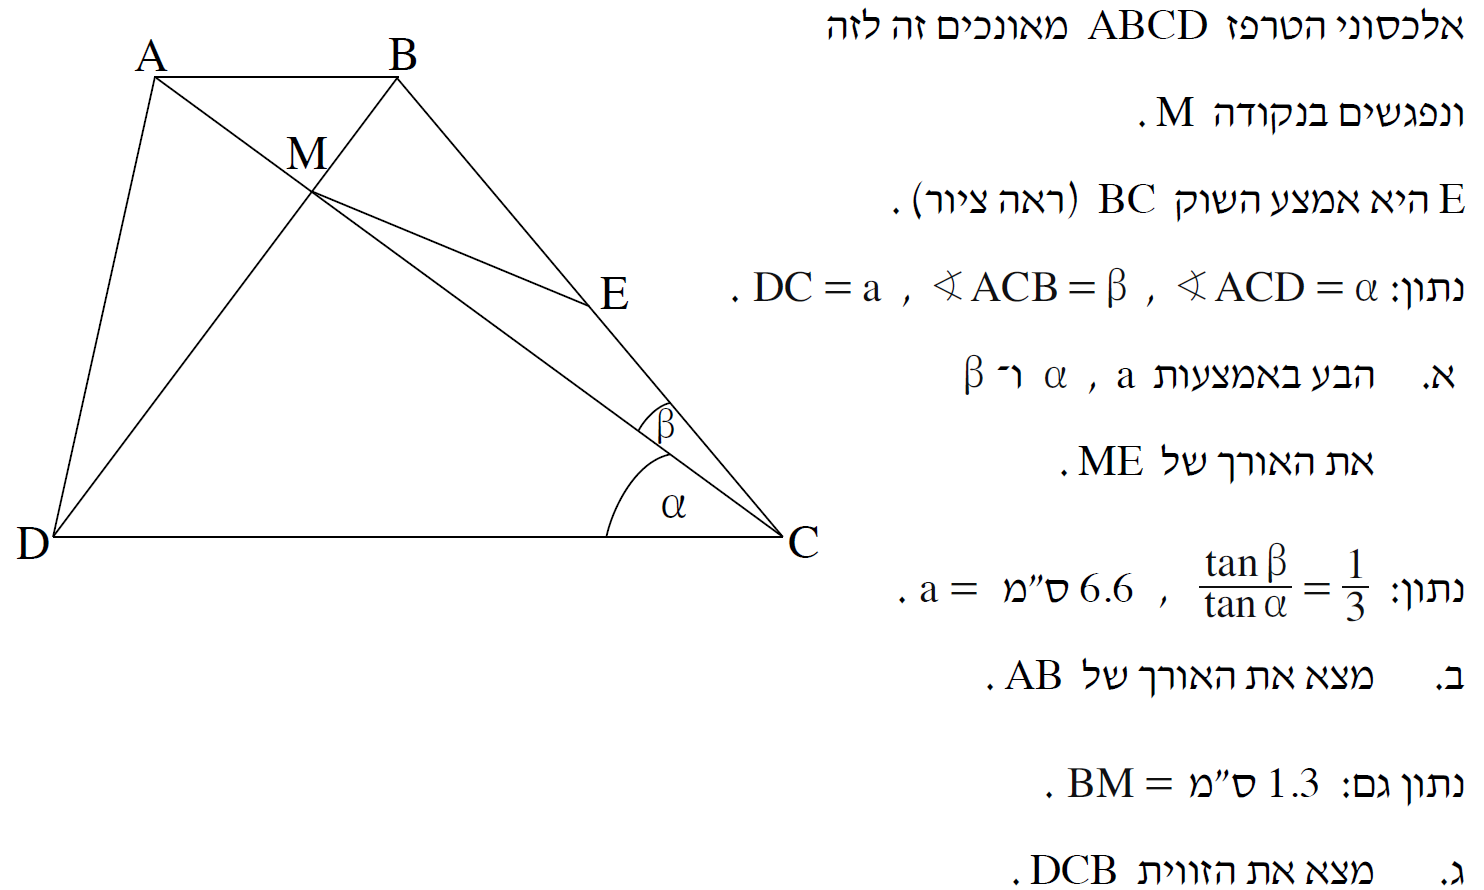
\includegraphics[width=.95\textwidth]{winter-2015-5}
\end{center}

\vspace{-1ex}

\textbf{סעיף א}

נמסן את הצלעות בתרשים.
\begin{center}
\selectlanguage{english}
\begin{tikzpicture}[scale=1.1]
\draw[thick] (0,0) coordinate (D) node[left] {$D$} -- node[below] {$a$} (6,0) coordinate (C) node[right] {$C$};
\draw[thick,name path=ca] (C) -- +(144:7) coordinate (A) node[left] {$A$};
\draw[thick,name path=db] (D) -- +(54:5.1) coordinate (B) node[right] {$B$};
\draw[thick] (D) -- (A) -- node[above] {$d$} (B) -- (C);
\path[name intersections={of=ca and db,by=M}];
\fill (A) node[below right,xshift=10pt] {$\alpha$} circle(1.5pt);
\fill (B) circle(1.5pt);
\fill (C) node[above left,xshift=-12pt] {$\alpha$} node[above left,xshift=-29pt,yshift=28pt] {$\beta$}  circle(1.5pt);
\fill (D) circle(1.5pt);
\fill (M) node[left,xshift=-2pt,yshift=-2pt] {$M$} circle(1.5pt);
\draw[rotate=-126] (M) rectangle +(8pt,8pt);
\coordinate (E) at ($(B) ! .5 ! (C) $);
\fill (E) node[right] {$E$} circle(1.5pt);
\draw[thick] (M) -- node[above] {$c/2$} (E);
\path (B) -- node[right] {$c/2$} (E) -- node[right] {$c/2$} (C);
\path (M) -- node[below] {$b$} (C);
\path (M) -- node[above] {$e$} (B);
\path (D) -- node[above] {$f$} (M);
\end{tikzpicture}
\end{center}

\vspace{-1ex}

נתון ש-%
$\angle BMC=90$
ולכן 
$\triangle BMC$
ישר זווית, ונתון ש-%
$ME$
הוא תיכון ליתר. מייד יש לנו
$ME=c/2$
לפי משפט 
$86$
"במשולש ישר זווית התיכון ליתר שווה למחצית היתר".


$ME=\displaystyle\frac{c}{2}=\frac{1}{2}\cdot \frac{b}{\cos \beta}$.
אבל
$b$
צלע משותף ל-%
$\triangle DMC,\triangle MEC$,
$ b = a\cos \alpha$.
מכאן ש:
\[
ME = \frac{c}{2} = \frac{b}{2\cos \beta} = \frac{a\cos \alpha}{2\cos \beta}\,.
\]

\np

\textbf{סעיף ב}

למשולשים
$\triangle AMB, \triangle CMB$
צעל משותף
$MB=e$.
\erh{12pt}
\begin{equationarray*}{rcl}
\tan \beta &=& \frac{e}{b}\\
\sin \alpha &=& \frac{e}{d}\\
AB = d &=& \frac{b\tan \beta}{\sin \alpha}\\
&=& \frac{a \cos\alpha\tan\beta}{\sin\alpha}\\
&=& \frac{a\tan\beta}{\tan\alpha}\\
&=& 6.6\cdot\frac{1}{3} = 2.2\,.
\end{equationarray*}
הוכחת אחרת משתמשת במשולשים דומים. 
$\angle BAM = \angle ACD = \alpha$
לפי זוויות מתחלפות, ו-%
$\triangle ABM \sim \triangle DMC$.
\erh{12pt}
\begin{equationarray*}{rcl}
\tan \beta &=& \frac{e}{b}\\
\tan \alpha &=& \frac{f}{b}\\
\frac{\tan \beta}{\tan \alpha} &=& \frac{e}{f}=\frac{1}{3}\\
\frac{d}{a}&=& \frac{1}{3}\\
AB = d&=& \frac{6.6}{3}=2.2\,.
\end{equationarray*}

\textbf{סעיף ג}
ממשפט פיתגורס
$b= \sqrt{a^2-f^2}=5.32$
ו:
\erh{12pt}
\begin{equationarray*}{rcl}
\tan \beta &=& \frac{e}{b} = \frac{1.3}{5.32}=0.2444\\
\beta &=& 13.73\\
\tan \alpha &=& 3\tan\beta = 0.7331\\
\alpha &=& 36.24\\
\angle DCB &=& \alpha + \beta = 49.97\,.
\end{equationarray*}



%%%%%%%%%%%%%%%%%%%%%%%%%%%%%%%%%%%%%%%%%%%%%%%%%%%%%%%%%%%%%%

\np

\section{קיץ תשע"ד מועד ב}

\begin{center}
\selectlanguage{english}
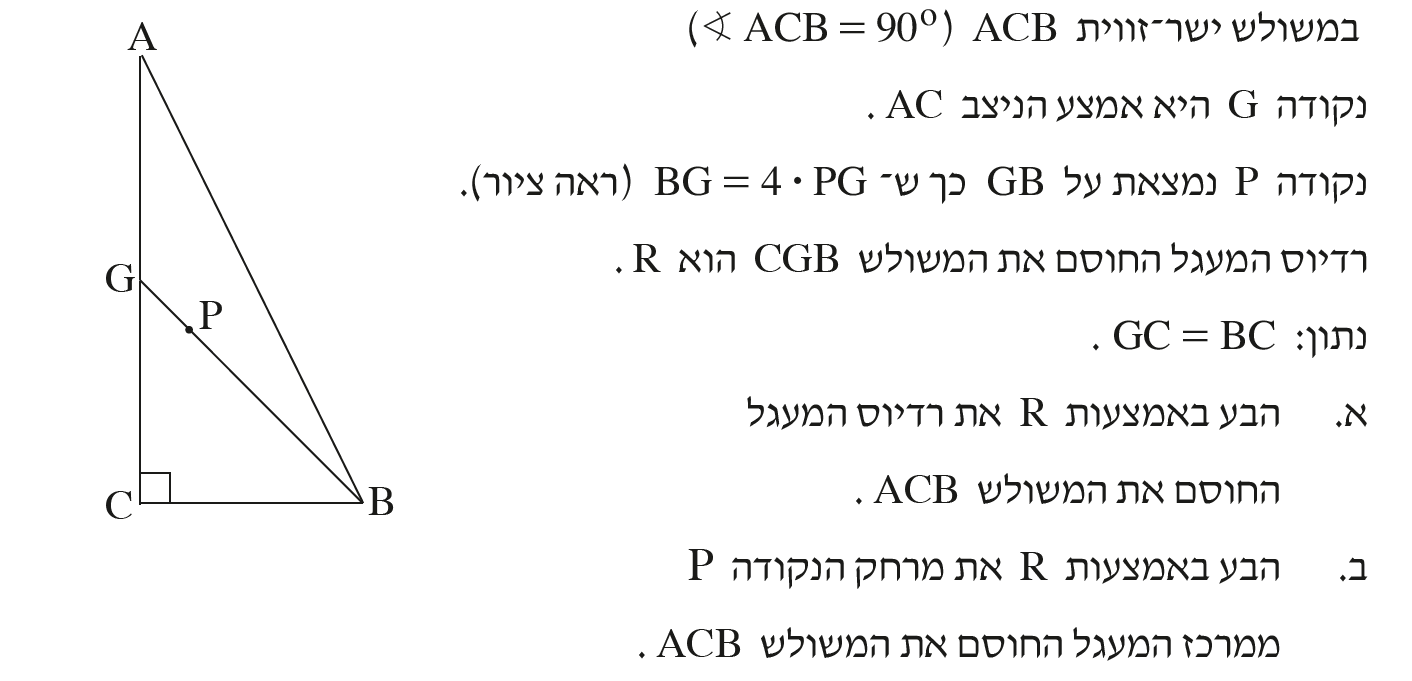
\includegraphics[width=\textwidth]{summer-2014b-5}
\end{center}

\vspace{-2ex}

\textbf{סעיף א}

\begin{center}
\selectlanguage{english}
\begin{tikzpicture}[scale=.8]
\draw[thick] (0,0) coordinate (C) -- node[below] {$a$} (4,0) coordinate (B) -- (0,8) coordinate (A) -- cycle;
\coordinate (G) at (0,4);
\path (C) -- node[left] {$a$} (G) -- node[left] {$a$} (A);
\draw[thick] (B) -- (G);
\coordinate (P) at ($(G)!.25!(B)$);
\fill (B) node[right] {$B$} circle(1.5pt);
\fill (A) node[above] {$A$} circle(1.5pt);
\fill (C) node[left] {$C$} circle(1.5pt);
\fill (G) node[left] {$G$} circle(1.5pt);
\fill (P) node[above,yshift=2pt] {$P$} circle(1.5pt);
\tkzCircumCenter(A,B,C)\tkzGetPoint{M1}
\tkzDrawCircle[thick,dotted,name path=circle](M1,A)
\tkzCircumCenter(C,G,B)\tkzGetPoint{M2}
\tkzDrawCircle[thick,dotted,name path=circle](M2,B)
\fill (M1) node[right] {$M'$} circle(1.5pt);
\fill (M2) node[left] {$M$} circle(1.5pt);
\draw (C) rectangle +(8pt,8pt);
\end{tikzpicture}
\end{center}

\vspace{-11ex}
נסמן
$=R,M$
את מרכז המעגל החוסם את
$CGB$
והרדיוס שלו, ו-%
$=R',M'$
את מרכז המעגל החוסם את
$ACB$
והרדיוס שלו.

נתון היחס בין הצלעות של המשולשים
$\triangle CGB, \triangle ACB$,
ולכן אפשר להשתמש בחוק הסינוסים ובמשפט פיתגורס, תחילה עבור
$\triangle CGB$:
\[
2R=\frac{BG}{\sin 90}=BG=\sqrt{a^2+a^2}=\sqrt{2}a\,,
\]

\np

ואחר כך עבור
$\triangle ACB$:
\[
2R'=\frac{AB}{\sin 90}=AB=\sqrt{a^2+(2a)^2}=\sqrt{5}a=\frac{\sqrt{5}}{\sqrt{2}}\cdot\sqrt{2}a=\sqrt{\frac{5}{2}}\cdot 2R\,,
\]
ולכן:
\[
R'=\sqrt{\frac{5}{2}}R\,.
\]

\textbf{סעיף ב}

מרכז המעגל החוסם הוא נקודת החיתוך של האנכים האמצעיים:
\[
GM'\perp AC,\quad M'H\perp BC,\quad CH=HB=\frac{a}{2}\,.
\]

\vspace{-4ex}

\begin{center}
\selectlanguage{english}
\begin{tikzpicture}[scale=1.4]
\clip (-.5,-1) rectangle +(5,5.4);
\draw[thick] (0,0) coordinate (C) -- (4,0) coordinate (B) -- (0,8) coordinate (A) -- cycle;
\coordinate (G) at (0,4);
\path (C) -- node[left] {$a$} (G) -- node[left] {$a$} (A);
\draw[thick] (B) -- (G);
\coordinate (P) at ($(G)!.25!(B)$);
\fill (B) node[right] {$B$} circle(1.5pt);
\fill (A) node[above] {$A$} circle(1.5pt);
\fill (C) node[left] {$C$} circle(1.5pt);
\fill (G) node[left] {$G$} circle(1.5pt);
\fill (P) node[below,xshift=-2pt,yshift=-2pt] {$P$} circle(1.5pt);
\tkzCircumCenter(A,B,C)\tkzGetPoint{M1}
%\tkzDrawCircle[thick,dotted,name path=circle](M1,A)
\tkzCircumCenter(C,G,B)\tkzGetPoint{M2}
%\tkzDrawCircle[thick,dotted,name path=circle](M2,B)
\fill (M1) node[right] {$M'$} circle(1.5pt);
\fill (M2) node[left,xshift=-2pt,yshift=-2pt] {$M$} circle(1.5pt);
\draw (C) rectangle +(8pt,8pt);
\draw (G) rectangle +(8pt,8pt);
\draw[thick] (P) -- node[above,xshift=-2pt] {$z$} (M1);
\coordinate (H) at (M1 |- B);
\fill (H) node[above left] {$H$} circle(1.5pt);
\draw[thick,dashed] (G) -- (M1) -- (H);
\draw (H) rectangle +(8pt,8pt);
\path (G) -- node[below,xshift=-4pt,yshift=2pt] {$x$} (P) -- node[below,xshift=-4pt,yshift=2pt] {$x$} (M2) -- node[below,xshift=-4pt,yshift=2pt] {$2x$} (B);
\path (C) -- node[below] {$a/2$} (H) -- node[below] {$a/2$} (B);
\path (M1) -- node[right] {$y$} (M2) -- node[left] {$a/2$} (H);
\end{tikzpicture}
\end{center}

\vspace{-5ex}

בסעיף הקודם חישבנו את האורך
$a$
כתלות ב-%
$R$,
וגם נתון היחס 
$BG=4\cdot PG$.
אם נמצא משולש שעבורו נוכל לחשב שני צלעות והזווית הכלואה ביניהם, נוכל להשתמש בחוק הקוסינוסים. בתרשים נראה ש-%
$\triangle MPM'$
יכול להתאים.

נסמן
$x=PM$, $y=MM'$, $z=PM'$.

לפי משפט 
$91$
"משפט תאלס המורחב: ישר המקביל לאחת מצלעות המשולש חותך את שתי הצלעות האחרות או את המשכיהן בקטעים פרופורציוניים." 
$CG\|MH$
ולכן:
\[
\frac{GB}{MB}=\frac{GC}{MH}=2\,.
\]
אבל
$GCHM'$
הוא מלבן ולכן
$y=MM'=\frac{a}{2}$.

ביחד עם הנתון
$GB=4\cdot PG$:
\[
MB=2x,\; GM = 2x,\; GP = PM =x\,,
\]
כפי שסומן בתרשים. את
$x$
ניתן לחשב לפי משפט פיתגורס:
\[
4x=4\cdot PM= GB= \sqrt{a^2+a^2}=\sqrt{2}a=2R,\quad x=\frac{R}{2}\,.
\]

\np

$\triangle MHB$
הוא ישר-זווית שווה-שוקיים, כך ש-%
$\angle PMM'=\angle BMH=45$
לפי זוויות קודקודיות.

כעת יש לנו מספיק נתונים להשתמש בחוק הקוסינוסים כי:
\[
x=\frac{R}{2},\quad y = \frac{a}{2} = \frac{2R}{2\sqrt{2}}=\frac{R}{\sqrt{2}}\,.
\]
\vspace{-10ex}

\erh{14pt}
\begin{equationarray*}{rcl}
z^2&=&x^2+y^2-2xy\cos \angle PMM'\\
&=&\frac{R^2}{4}+\frac{R^2}{2} - 2\frac{R}{2}\frac{R}{\sqrt{2}}\cos 45\\
&=& R^2(\frac{1}{4}+\frac{1}{2}-\frac{\sqrt{2}}{2\sqrt{2}})\\
&=&\frac{R^2}{4}\\
PG=z&=&\frac{R}{2}\,.
\end{equationarray*}

$M'$,
מרכז המעגל החוסם את
$ACB$
מסומן על הצלע
$AB$.
הטענה נכונה, אבל להוכחנו אותה וגם לא השתמשנו בה בפתרון. קיימת פתרון לשאלה אם נוכיח את הטענה.

האנך האמצעי
$GM'$
מקביל לצעל
$CB$
ולפי משפט תאלס המורחב חוצה את הצלע
$AB$.
מכאן שהאנך האמצעי של 
$AB$
חותך את 
$AB$
ב-%
$M'$
והוא המרכז של המעגל החוסם.

נסמן
$y=AB$,
$4x=GB$,
$PM'=z$,
$\alpha = \angle CAB$,
$\beta = \angle ABG$.
מסעיף א יש לנו
\[
a = \sqrt{2}R,\quad 4x=2R,\quad y=2\sqrt{\frac{5}{2}}R=\sqrt{10}R\,.
\]
\begin{center}
\selectlanguage{english}
\begin{tikzpicture}[scale=.8]
\draw[thick] (0,0) coordinate (C) -- node[below] {$a$} (4,0) coordinate (B) -- (0,8) coordinate (A) node[below,xshift=6pt,yshift=-20pt] {$\alpha$} -- cycle;
\coordinate (G) at (0,4);
\path (C) -- node[left] {$a$} (G) -- node[left] {$a$} (A);
\draw[thick] (B) -- (G);
\coordinate (P) at ($(G)!.25!(B)$);
\fill (B) node[right] {$B$} circle(1.5pt);
\fill (A) node[above] {$A$} circle(1.5pt);
\fill (C) node[left] {$C$} circle(1.5pt);
\fill (G) node[left] {$G$} node[below,xshift=8pt,yshift=-12pt] {$45$} circle(1.5pt);
\fill (P) node[below,yshift=-2pt] {$P$} circle(1.5pt);
\tkzCircumCenter(A,B,C)\tkzGetPoint{M1}
%\tkzDrawCircle[thick,dotted,name path=circle](M1,A)
\tkzCircumCenter(C,G,B)\tkzGetPoint{M2}
%\tkzDrawCircle[thick,dotted,name path=circle](M2,B)
\fill (M1) node[right] {$M'$} circle(1.5pt);
%\fill (M2) node[left] {$M$} circle(1.5pt);
\draw (C) rectangle +(8pt,8pt);
\draw (G) rectangle +(8pt,8pt);
\draw[thick,dashed] (G) -- (M1);
\draw[thick] (P) -- (M1);
\path (A) -- node[right] {$y/2$} (M1) -- node[right] {$y/2$} (B);
\node at ($(B)+(15pt,20pt)$) {$\beta$};
\draw[->] ($(B)+(10pt,20pt)$) -- +(-26pt,0);
\path (P) -- node[below,near start,yshift=-2pt] {$3x$} (B);
\path (P) -- node[above,near start] {$z$} (M1);
\end{tikzpicture}
\end{center}
נחשב את הזוויות
$\alpha,\beta$
ונשמתש בחוק הקוסינוסים:
\erh{14 pt}
\begin{equationarray*}{rcl}
\sin \alpha &=& \frac{a}{y}= \frac{\sqrt{2}R}{\sqrt{10}R} = \sqrt{\frac{1}{5}}\\
\alpha &=& 26.57\\
\beta&=& 180-\angle AGB-\alpha=180-135-26.57=18.43\\
z^2&=&(3x)^2 + \frac{y}{2}^2 - 2\cdot 3x\cdot \frac{y}{2} \cdot \cos 18.43\\
&=&\left(\frac{3R}{2}\right)^2 + \left(\frac{\sqrt{10}R}{2}\right)^2 - 2\cdot \frac{3R}{2} \cdot \frac{\sqrt{10}R}{2} \cdot 0.9487\\
&=&0.25R^2\\
PM'=z&=&\frac{R}{2}\,.
\end{equationarray*}
אני מעדיף את הפתרון הראשון. אמנם התרשים מעט יותר מסובך אבל החישובים הרבה יותר פשוטים.



\np

\section{קיץ תשע"ד מועד א}

%%%%%%%%%%%%%%%%%%%%%%%%%%%%%%%%%%%%%%%%%%%%%%%%%%%%%%%%%%%%%%

\begin{center}
\selectlanguage{english}
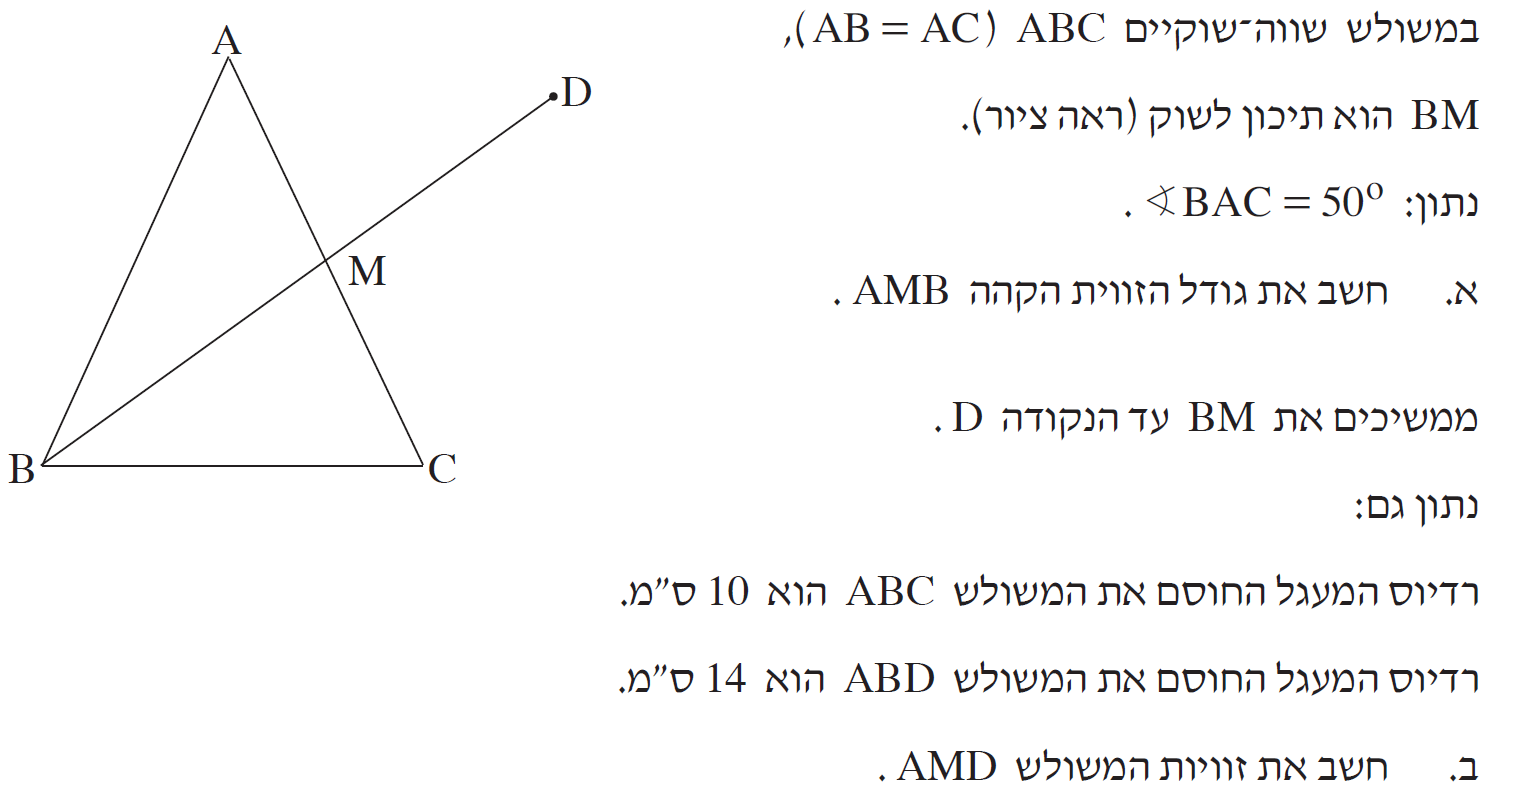
\includegraphics[width=\textwidth]{summer-2014a-5}
\end{center}

\textbf{סעיף א}

נסמן את הזווית המבוקשת
$\alpha=\angle AMB$.
נתון 
$\angle BAC=50$
ובמשולש שווה-שוקיים:
\[
\angle ABC=\angle ACB=(180-50)/2=65\,.
\]
\begin{center}
\selectlanguage{english}
\begin{tikzpicture}[scale=.9]
\draw[thick] (0,0) coordinate (B) -- (5,0) coordinate (C);
\draw[thick] (B) -- node[left] {$a$} (2.5,6) coordinate (A);
\draw[thick,name path=ac] (A) -- (C);
\fill (B) node[below left] {$B$} node[above right,xshift=4pt] {$65$} circle(1.5pt);
\fill (A) node[above] {$A$} node[below,yshift=-16pt] {$50$} circle(1.5pt);
\fill (C) node[below right] {$C$} node[above left,xshift=-4pt] {$65$} circle(1.5pt);
\coordinate (M) at ($(A)!.5!(C)$);
\fill (M) node[below right,xshift=4pt,yshift=2pt] {$M$} node[left,yshift=2pt] {$\alpha$}  circle(1.5pt);
\draw[thick] (B) -- ($(B)!1.5!(M)$) coordinate (D);
\fill (D) node[right] {$D$} circle(1.5pt);
\path (A) -- node[right] {$a/2$} (M);
\path (M) -- node[right] {$a/2$} (C);
\node at ($(B)+(-25pt,25pt)$) {$130\!-\!\alpha$};
\draw[->] ($(B)+(0,25pt)$) -- +(18pt,0);
\end{tikzpicture}
\end{center}
בדיקה קצרה מראה שאין מספיק נתונים לחשב את הזוויות רק מהשלמת הזוויות.

נתון ש-%
$BM$
הוא תיכון ל-%
$AC$
וסמנו את אורכי הצלעות בנעלם
$a$.
אם נפעיל את משפט הסינוים על המשולש
$\triangle ABM$,
הנעלם יצטמצם:

\np

\erh{12pt}
\begin{equationarray*}{rcl}
\frac{a}{\sin\alpha}&=&\frac{a/2}{\sin(130-\alpha)}\\
\sin \alpha &=& 2\sin(130-\alpha)\\
&=&2\sin 130\cos \alpha - 2\sin\alpha \cos 130\\
&=&1.53\cos\alpha + 1.29\sin\alpha\\
\tan \alpha &=& \frac{-1.53}{0.29}\\
\tan(180-\alpha) &=& \frac{1.53}{0.29}\\
\alpha&=&100.73^\circ\approx 101^\circ\,.
\end{equationarray*}
$\tan(180-\alpha)=-\tan\alpha$
כי הסימן הקוסינוס מתחלף והסימן הסינוס נשאר אותו דבר.

\medskip

\textbf{סעיף ב}

\vspace{-12ex}

\begin{center}
\selectlanguage{english}
\begin{tikzpicture}[scale=.9]
\draw[thick] (0,0) coordinate (B) -- (5,0) coordinate (C);
\draw[thick] (B) -- node[left] {$a$} (2.5,6) coordinate (A);
\draw[thick,name path=ac] (A) -- (C);
\fill (B) node[below left] {$B$} node[above right,xshift=11pt,yshift=20pt] {$29$} node[above right,xshift=16pt] {$36$} circle(1.5pt);
\fill (A) node[above] {$A$} node[below,yshift=-16pt] {$50$} circle(1.5pt);
\fill (C) node[below right] {$C$} node[above left,xshift=-4pt] {$65$} circle(1.5pt);
\coordinate (M) at ($(A)!.5!(C)$);
\fill (M) node[below right,xshift=4pt,yshift=2pt] {$M$} node[left,yshift=2pt] {$101$} node[above,xshift=3pt,yshift=7pt] {$79$}  circle(1.5pt);
\draw[thick] (B) -- ($(B)!1.8!(M)$) coordinate (D);
\fill (D) node[right] {$D$} node[below left,xshift=-12pt,yshift=2pt] {$\beta$} circle(1.5pt);
\path (A) -- (M);
\path (M) -- (C);
\tkzCircumCenter(A,B,C)\tkzGetPoint{C1}
\tkzDrawCircle[thick,dotted,name path=circle](C1,A)
\tkzCircumCenter(A,B,D)\tkzGetPoint{D1}
\tkzDrawCircle[thick,dotted,name path=circle](D1,A)
\draw[thick,dashed] (A) -- (D);
\end{tikzpicture}
\end{center}
את הזווית
$\angle AMD$
חישבנו בסעיף הקודם. נצטרך לחשב אחת מהזוויות
$\angle MAD,\angle ADM$
והזווית השלישית תתקבל מסכום הזוויות במשולש. מהתרשים אנו רואים שהצלע מול הזווית
$\beta=\angle MAD$
הוא באורך
$a$,
ואותו צלע הוא מול הזווית
$\angle AMB=101$.
לפי חוק הסינוסים:

\np

\erh{12pt}
\begin{equationarray*}{rcl}
2R_{ABC}&=&\frac{a}{\sin 65}=2\cdot 10\\
2R_{ABD}&=&\frac{a}{\sin \beta}=2\cdot 14\\
a &=& 18.126\\
\sin \beta &=& 0.647\\
\beta &=& 40.34\,.
\end{equationarray*}
שלושת הזוויות של
$\triangle AMD$
הן )בקירוב למעלה שלמה(
$79^\circ, 40^\circ, 61^\circ$.


%%%%%%%%%%%%%%%%%%%%%%%%%%%%%%%%%%%%%%%%%%%%%%%%%%%%%%%%%%%%%%
\np

\section{חורף תשע"ד}

\begin{center}
\selectlanguage{english}
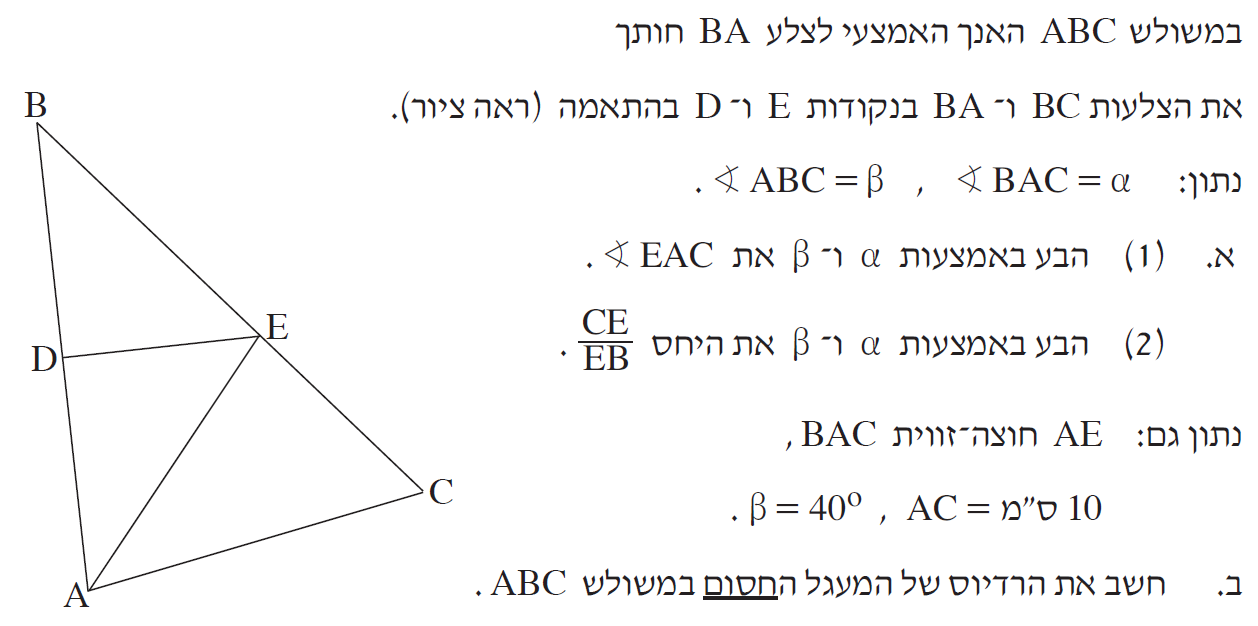
\includegraphics[width=\textwidth]{winter-2014-5}
\end{center}

\textbf{סעיף א}

נתון ש-%
$DE$
הוא האנך האמצעי ל-%
$AB$,
ולכן
$\triangle AED\cong BED$.
לא נותר אלא לסמן זוויות לפי זווית משלימה וסכום זוויות המשולש. )קיצרנו
$\beta'=90-\beta$.(
$\angle EAC=\alpha-\beta$.

\begin{center}
\selectlanguage{english}
\begin{tikzpicture}[scale=.9]
\draw[thick] (0,0) coordinate (A) -- (5,1) coordinate (C);
\draw[thick] (A) -- (100:8) coordinate (B);
\draw[thick,name path=bc] (B) -- (C);
\coordinate (D) at ($(A) ! .5 ! (B)$);
\fill (A) node[below left] {$A$} node[above right,xshift=14pt,yshift=12pt] {$\alpha-\beta$} node[above,xshift=2pt,yshift=16pt] {$\beta$} circle(1.5pt);
\fill (B) node[above] {$B$} node[below right,xshift=4pt,yshift=-14pt] {$\beta$} circle(1.5pt);
\fill (C) node[right] {$C$} node[above right,xshift=-4pt,yshift=6pt] {$180-(\alpha+\beta)$} circle(1.5pt);
\draw[->] ($(C)+(0pt,12pt)$) -- +(-14pt,-8pt);
\fill (D) node[left] {$D$} circle(1.5pt);
\path[name path=de] (D) -- +(10:4);
\path[name intersections={of=bc and de,by={E}}];
\fill (E) node[right] {$E$} node[above left,xshift=-8pt,yshift=-4pt] {$\beta'$} node[below left] {$\beta'$} node[below,xshift=4pt,yshift=-12pt] {$2\beta$}   circle(1.5pt);
\draw[thick] (D) -- (E);
\draw[thick,name path=ae] (A) -- (E);
\path (A) -- node[left] {$a$} (D);
\path (D) -- node[left] {$a$} (B);
\path (C) -- node[right] {$c$} (E);
\path (E) -- node[right,xshift=2pt] {$b$} (B);
\path (E) -- node[right] {$b$} (A);
\draw[rotate=10] (D) rectangle +(7pt,7pt);
\draw[thick] ($(A)+(10:8mm)$) arc[start angle=25,end angle=101,radius=8mm];
\end{tikzpicture}
\end{center}

\np

\textbf{סעיף ב}

בתרשים שני הקטעים מסומנים ב-%
$b,c$
והשאלה מבקש את היחס
$\frac{c}{b}$.
המחשבה הראשונה היתה להשתמש במשפט תאלס אבל לא ידוע ש-%
$DE\not\|AC$.
השאלה עוסקת בטריגונומטריה אז ננסה את משפט הסינוסים. בסעיף הקודם ראינו ש-%
$\triangle AED\cong BED$
ואם נסמן גם
$AE=b$,
נוכל להשתמש במשפט ב-%
$\triangle AEC$:
\[
\frac{c}{\sin (\alpha-\beta)}=\frac{b}{\sin(180-(\alpha+\beta))}\,.
\]
מבט במעגל היחידה מראה ש-%
$\sin (180-\theta) = \sin \theta$,
ולכן
\[
\frac{c}{b}=\frac{\sin (\alpha-\beta)}{\sin (\alpha+\beta)}\,.
\]
\begin{center}
\selectlanguage{english}
% Functions of 180-\theta
\begin{tikzpicture}[scale=1.8]
\coordinate (origin) at (0,0);
% Draw circle
\draw[name path=circle] (origin) circle [radius=1];
% Draw axes
\draw (-1,0) -- (1,0);
\draw (0,-1) -- (0,1);
% Draw first ray
\path[name path=ray1] (origin) -- +(40:1.1);
\path[name intersections={of=circle and ray1,by=on-circle1}];
\draw (origin) node[above right,xshift=18pt,yshift=-1pt] {$\theta$} -- (on-circle1) node[above right,xshift=-4pt] {$(\cos \theta, \sin \theta)$};
% Draw altitude and square for right angle
\draw[dashed] (on-circle1) -- (on-circle1 |- origin);
\draw (on-circle1 |- origin) rectangle +(-2pt,2pt);
% Draw second ray
\path[name path=ray2] (origin) -- +(140:1.1);
\path[name intersections={of=circle and ray2,by=on-circle2}];
\draw (origin) -- (on-circle2) node[above left,xshift=4pt] {$(-\cos \theta, \sin \theta)$};
% Draw altitude and square for right angle
\draw[dashed] (on-circle2) -- (on-circle2 |- origin);
\draw (on-circle2 |- origin) rectangle +(2pt,2pt);
% Draw the arc for 180-\theta
\draw (12pt,0) arc(0:140:12pt);
\node at (8pt,18pt) {$180-\theta$};
\draw[->] (6pt,15pt) -- +(0,-4pt);
\end{tikzpicture}
\end{center}

\textbf{סעיף ג}

המשפט הרלוונטי למעגל חסום הוא
$49$
"שלושת חוצי הזוויות של משולש נחתכים בנקודה אחת, שהיא מרכז המעגל החסום במשולש". נתון חוצה זווית אחד ב-%
$A$.
לא ברור מראש אם כדאי לבדוק את החיתוך עם חוצה הזווית ב-%
$B$
או ב-%
$C$.
ננסה ב-%
$C$
כי אנחנו צריכים אורך )של הרדיוס( ונתון לנו
$AC=10$,
$\beta=40^\circ$,
וש-%
$AE$
הוא חוצה זווית, וזה מאפשר לנו לסמן ערכים:
\begin{center}
\selectlanguage{english}
\begin{tikzpicture}[scale=.9]
\draw[thick] (0,0) coordinate (A) -- (5,1) coordinate (C);
\draw[thick] (A) -- (100:8) coordinate (B);
\draw[thick,name path=bc] (B) -- (C);
\coordinate (D) at ($(A) ! .5 ! (B)$);
\fill (A) node[below left] {$A$} node[above right,xshift=10pt,yshift=10pt] {$40$} node[above,xshift=3pt,yshift=18pt] {$40$} circle(1.5pt);
\fill (B) node[above] {$B$} node[below right,xshift=3pt,yshift=-18pt] {$40$} circle(1.5pt);
\fill (C) node[right] {$C$} node[left,xshift=-14pt,yshift=2pt] {$30$} node[above left,xshift=-16pt,yshift=8pt] {$30$} circle(1.5pt);
%\draw[->] ($(C)+(0pt,12pt)$) -- +(-14pt,-8pt);
\fill (D) node[left] {$D$} circle(1.5pt);
\path[name path=de] (D) -- +(10:4);
\path[name intersections={of=bc and de,by={E}}];
\fill (E) node[right] {$E$} node[above left,xshift=-8pt,yshift=-4pt] {$50$} node[below left,xshift=-3pt,yshift=-2pt] {$50$} node[below,xshift=4pt,yshift=-12pt] {$80$}   circle(1.5pt);
\draw[thick] (D) -- (E);
\draw[thick,name path=ae] (A) -- (E);
\path (A) -- node[left] {$a$} (D);
\path (D) -- node[left] {$a$} (B);
\path (C) -- node[right] {$c$} (E);
\path (E) -- node[right,xshift=2pt] {$b$} (B);
\path (E) -- node[right,xshift=4pt,yshift=10pt] {$b$} (A);
\path (A) -- node[below] {$10$} (C);
\draw[rotate=10] (D) rectangle +(7pt,7pt);
%\draw[thick] ($(A)+(10:8mm)$) arc[start angle=25,end angle=101,radius=8mm];
\path[name path=cf] (C) -- +(160:5);
\path[name intersections={of=ae and cf,by={F}}];
\fill (F) node[left] {$F$} node[below,xshift=8pt,yshift=-8pt] {$110$} circle(1.5pt);
\draw[thick] (C) -- node[above] {$x$} (F);
\end{tikzpicture}
\end{center}
\np
הנקודה
$F$
היא נקודת החיתוך של חוצי הזוויות ולכן היא מרכז המעגל החסום. לפי משפט הסינוסים:
\erh{14pt}
\begin{equationarray*}{rcl}
\frac{x}{\sin 40}&=&\frac{10}{\sin 110}\\
x &=& \frac{10\sin 40}{\sin 110} = 6.84\,.
\end{equationarray*}
\textbf{לא לעצור כאן!}
השאלה מבקשת את הרדיוס של המעגל החסום ולא המרחק של מרכז המעגל. 

נוריד אנך לצלע 
$AC$
ונוכל לחשב:
\[
r=x\sin 30 = \frac{6.84}{2} = 3.42\,.
\]
כדי להראות את המעגל החסום, ציירתי תרשים חדש עם ערכי זוויות מדוייקים:
\begin{center}
\selectlanguage{english}
\begin{tikzpicture}[scale=.9]
\coordinate (A) at (0,0);
\draw[thick] (A) -- +(90:8) coordinate (B);
\path[name path=bc] (B) -- +(-50:10);
\path[name path=ac] (A) -- +(10:7);
\path[name intersections={of=ac and bc,by={C}}];
\draw[thick] (A) -- (C) -- (B);
\fill (B) node[above] {$B$};
\fill (A) node[below left] {$A$} node[above right,xshift=10pt,yshift=4pt] {$40$} circle(1.5pt);
\fill (C) node[right] {$C$} node[left,xshift=-14pt,yshift=2pt] {$30$} circle(1.5pt);
\path[name path=af] (A) -- +(50:5);
\path[name path=cf] (C) -- +(160:6);
\path[name intersections={of=af and cf,by={F}}];
\fill (F) node[above] {$F$} circle(1.5pt);
\draw[thick] (A) -- (F) -- node[above,near start] {$x$} (C);
\coordinate (G) at ($(A)!(F)!(C)$);
\draw[very thick,dashed]  (G) -- node[left] {$r$} (F);
\draw[rotate=10] (G) rectangle +(7pt,7pt);
\fill (G) circle(1.5pt);
\node[draw,very thick,dotted,circle through=(G)] at (F) {};
\end{tikzpicture}
\end{center}


\np

\section{המלצות}

\begin{itemize}

\item
כצעד ראשון בפתרון בעייה, סמנו את הזוויות שיש למצוא אותן באות יוונית
$\alpha,\beta,\ldots$.
השלימו זוויות ככל האפשר תוך שימוש בסכום הזוויות במשולש, ובזוויות משלימות. כדי להקל על החישובים אני משתמש בנעלמים נוספים כדי לקצר ביטויים כגון
$\gamma=180-(\alpha+\beta)$.

\item
שימו לב שאין עקביות בסימון 
$A,B,C,D$
של הקודקודים של משולש או מרובע.


\item 
בשאלות על טריגונומטריה בדרך כלל עדיף להשתמש בנוסחה לשטח משולש:
\[
S=\frac{1}{2}\cdot b \cdot c \cdot\sin \alpha\,,
\]
ולא בחישוב של מחצית מכפלת הבסיס והגובה.

\item
עבור מעגל חוסם, המשפט הרלוונטי הוא
$54$
"במשולש, שלושת האנכים האמצעיים נחתכים בנקודה אחת , שהיא מרכז המעגל החוסם את המשולש". ניתן בקלות למצוא את רדיוס המעגל מחוק הסינוסים:
\[
2R=\frac{a}{\sin\alpha}\,.
\]
\vspace{-4ex}
\item
עבור מעגל חסום, המשפט הרלוונטי הוא
$49$
"שלושת חוצי הזוויות של משולש נחתכים בנקודה אחת, שהיא מרכז המעגל החסום במשולש". אין נוסחה עבור רדיוס המעגל אבל אפשר למצוא אותו כאורך הגובה מהמרכז לאחד הצלעות.


\item 
טרפזים מאוד אהובים על ידי כותבי הבחינה. שננו משפטים
$56$
"ניתן לחסום מרובע במעגל אם ורק אם סכום זוג זוויות נגדיות שווה ל-%
$180$"
ו-%
$57$
"מרובע קמור חוסם מעגל אם ורק אם סכום שתי צלעות נגדיות שווה לסכום שתי הצלעות הנגדיות האחרות".

\item
כאשר ידוע שתי זוויות של מעגל
$\alpha,\beta$,
 הזווית השלישית היא
$180-(\alpha+\beta)$.
ניתן להשמתמש בזהות )ראו נספח~%
\ref{a.unit-circle}(:
\[
\sin (180-\theta) = \sin \theta\,.
\]
\vspace{-5ex}

\item
במשולש ישר-זווית, אם יודעים את אחת הזוויות החדות 
$\alpha$
הזווית החדה שנייה היא
$90-\alpha$.
ניתן להשתמש בזהות:
\[
\sin (90-\theta) = \cos \theta\,.
\]
שימו לב לא להתבלבל ולכתוב
$\sin (90-\theta) = \sin\theta$
כמו במשולש רגיל.
\item
לעתים קרובות התשובה לשאלה תהיה ערך ממשי לזווית או אורך. אני מעדיף להישאר עם נעלמים כל עוד הדבר אפשרי ורק בסוף להשתמש במחשבון כדי לחשב ערכים.


\end{itemize}

\selectlanguage{english}

